\documentclass[10pt,a4paper,onecolumn]{article}
\usepackage{marginnote}
\usepackage{graphicx}
\usepackage[rgb,svgnames]{xcolor}
\usepackage{authblk,etoolbox}
\usepackage{titlesec}
\usepackage{calc}
\usepackage{tikz}
\usepackage[pdfa]{hyperref}
\usepackage{hyperxmp}
\hypersetup{%
    unicode=true,
    pdfapart=3,
    pdfaconformance=B,
    pdftitle={maze-dataset: Maze Generation with Algorithmic Variety and
Representational Flexibility},
    pdfauthor={Michael Igorevich Ivanitskiy, Aaron Sandoval, Alex F.
Spies, Tilman Räuker, Brandon Knutson, Cecilia Diniz Behn, Samy Wu
Fung},
    pdfpublication={Journal of Open Source Software},
    pdfpublisher={Open Journals},
    pdfissn={2475-9066},
    pdfpubtype={journal},
    pdfvolumenum={},
    pdfissuenum={},
    pdfdoi={N/A},
    pdfcopyright={Copyright (c) 1970, Michael Igorevich Ivanitskiy,
Aaron Sandoval, Alex F. Spies, Tilman Räuker, Brandon Knutson, Cecilia
Diniz Behn, Samy Wu Fung},
    pdflicenseurl={http://creativecommons.org/licenses/by/4.0/},
    colorlinks=true,
    linkcolor=[rgb]{0.0, 0.5, 1.0},
    citecolor=Blue,
    urlcolor=[rgb]{0.0, 0.5, 1.0},
    breaklinks=true
}
% https://tex.stackexchange.com/a/535849
% Create an OutputIntent in order to correctly specify colours
\immediate\pdfobj stream attr{/N 3} file{sRGB.icc}
\pdfcatalog{%
  /OutputIntents [
    <<
      /Type /OutputIntent
      /S /GTS_PDFA1
      /DestOutputProfile \the\pdflastobj\space 0 R
      /OutputConditionIdentifier (sRGB)
      /Info (sRGB)
    >>
  ]
}
\pdfvariable omitcidset=1
\usepackage{caption}
\usepackage{orcidlink}
\usepackage{tcolorbox}
\usepackage{amssymb,amsmath}
\usepackage{ifxetex,ifluatex}
\usepackage{seqsplit}
\usepackage{xstring}

\usepackage{float}
\let\origfigure\figure
\let\endorigfigure\endfigure
\renewenvironment{figure}[1][2] {
    \expandafter\origfigure\expandafter[H]
} {
    \endorigfigure
}

\usepackage{fixltx2e} % provides \textsubscript

% definitions for citeproc citations
\NewDocumentCommand\citeproctext{}{}
\NewDocumentCommand\citeproc{mm}{%
  \begingroup\def\citeproctext{#2}\cite{#1}\endgroup}
\makeatletter
 % allow citations to break across lines
 \let\@cite@ofmt\@firstofone
 % avoid brackets around text for \cite:
 \def\@biblabel#1{}
 \def\@cite#1#2{{#1\if@tempswa , #2\fi}}
\makeatother
\newlength{\cslhangindent}
\setlength{\cslhangindent}{1.5em}
\newlength{\csllabelwidth}
\setlength{\csllabelwidth}{3em}
\newenvironment{CSLReferences}[2] % #1 hanging-indent, #2 entry-spacing
 {\begin{list}{}{%
  \setlength{\itemindent}{0pt}
  \setlength{\leftmargin}{0pt}
  \setlength{\parsep}{0pt}
  % turn on hanging indent if param 1 is 1
  \ifodd #1
   \setlength{\leftmargin}{\cslhangindent}
   \setlength{\itemindent}{-1\cslhangindent}
  \fi
  % set entry spacing
  \setlength{\itemsep}{#2\baselineskip}}}
 {\end{list}}
\usepackage{calc}
\newcommand{\CSLBlock}[1]{\hfill\break\parbox[t]{\linewidth}{\strut\ignorespaces#1\strut}}
\newcommand{\CSLLeftMargin}[1]{\parbox[t]{\csllabelwidth}{\strut#1\strut}}
\newcommand{\CSLRightInline}[1]{\parbox[t]{\linewidth - \csllabelwidth}{\strut#1\strut}}
\newcommand{\CSLIndent}[1]{\hspace{\cslhangindent}#1}

% --- Page layout -------------------------------------------------------------
\usepackage[top=3.5cm, bottom=3cm, right=1.5cm, left=1.0cm,
            headheight=2.2cm, reversemp, includemp, marginparwidth=4.5cm]{geometry}

% --- Default font ------------------------------------------------------------
\renewcommand\familydefault{\sfdefault}

% --- Style -------------------------------------------------------------------
\renewcommand{\captionfont}{\small\sffamily}
\renewcommand{\captionlabelfont}{\bfseries}

% --- Section/SubSection/SubSubSection ----------------------------------------
\titleformat{\section}
  {\normalfont\sffamily\Large\bfseries}
  {}{0pt}{}
\titleformat{\subsection}
  {\normalfont\sffamily\large\bfseries}
  {}{0pt}{}
\titleformat{\subsubsection}
  {\normalfont\sffamily\bfseries}
  {}{0pt}{}
\titleformat*{\paragraph}
  {\sffamily\normalsize}


% --- Header / Footer ---------------------------------------------------------
\usepackage{fancyhdr}
\pagestyle{fancy}
\fancyhf{}
%\renewcommand{\headrulewidth}{0.50pt}
\renewcommand{\headrulewidth}{0pt}
\fancyhead[L]{\hspace{-0.75cm}
\includegraphics[width=5.5cm]{joss/logo.png}}
\fancyhead[C]{}
\fancyhead[R]{}
\renewcommand{\footrulewidth}{0.25pt}

\fancyfoot[L]{\parbox[t]{0.98\headwidth}{\footnotesize{\sffamily Ivanitskiy
et al. (1970). maze-dataset: Maze Generation with Algorithmic Variety
and Representational Flexibility. \emph{Journal of Open Source
Software}, \emph{¿VOL?}(¿ISSUE?), ¿PAGE? \url{https://doi.org/N/A}}.}}


\fancyfoot[R]{\sffamily \thepage}
\makeatletter
\let\ps@plain\ps@fancy
\fancyheadoffset[L]{4.5cm}
\fancyfootoffset[L]{4.5cm}

% --- Macros ---------

\definecolor{linky}{rgb}{0.0, 0.5, 1.0}

\newtcolorbox{repobox}
   {colback=red, colframe=red!75!black,
     boxrule=0.5pt, arc=2pt, left=6pt, right=6pt, top=3pt, bottom=3pt}

\newcommand{\ExternalLink}{%
   \tikz[x=1.2ex, y=1.2ex, baseline=-0.05ex]{%
       \begin{scope}[x=1ex, y=1ex]
           \clip (-0.1,-0.1)
               --++ (-0, 1.2)
               --++ (0.6, 0)
               --++ (0, -0.6)
               --++ (0.6, 0)
               --++ (0, -1);
           \path[draw,
               line width = 0.5,
               rounded corners=0.5]
               (0,0) rectangle (1,1);
       \end{scope}
       \path[draw, line width = 0.5] (0.5, 0.5)
           -- (1, 1);
       \path[draw, line width = 0.5] (0.6, 1)
           -- (1, 1) -- (1, 0.6);
       }
   }

\definecolor{c53baa1}{RGB}{83,186,161}
\definecolor{c202826}{RGB}{32,40,38}
\def \rorglobalscale {0.1}
\newcommand{\rorlogo}{%
\begin{tikzpicture}[y=1cm, x=1cm, yscale=\rorglobalscale,xscale=\rorglobalscale, every node/.append style={scale=\rorglobalscale}, inner sep=0pt, outer sep=0pt]
  \begin{scope}[even odd rule,line join=round,miter limit=2.0,shift={(-0.025, 0.0216)}]
    \path[fill=c53baa1,nonzero rule,line join=round,miter limit=2.0] (1.8164, 3.012) -- (1.4954, 2.5204) -- (1.1742, 3.012) -- (1.8164, 3.012) -- cycle;
    \path[fill=c53baa1,nonzero rule,line join=round,miter limit=2.0] (3.1594, 3.012) -- (2.8385, 2.5204) -- (2.5172, 3.012) -- (3.1594, 3.012) -- cycle;
    \path[fill=c53baa1,nonzero rule,line join=round,miter limit=2.0] (1.1742, 0.0669) -- (1.4954, 0.5588) -- (1.8164, 0.0669) -- (1.1742, 0.0669) -- cycle;
    \path[fill=c53baa1,nonzero rule,line join=round,miter limit=2.0] (2.5172, 0.0669) -- (2.8385, 0.5588) -- (3.1594, 0.0669) -- (2.5172, 0.0669) -- cycle;
    \path[fill=c202826,nonzero rule,line join=round,miter limit=2.0] (3.8505, 1.4364).. controls (3.9643, 1.4576) and (4.0508, 1.5081) .. (4.1098, 1.5878).. controls (4.169, 1.6674) and (4.1984, 1.7642) .. (4.1984, 1.8777).. controls (4.1984, 1.9719) and (4.182, 2.0503) .. (4.1495, 2.1132).. controls (4.1169, 2.1762) and (4.0727, 2.2262) .. (4.0174, 2.2635).. controls (3.9621, 2.3006) and (3.8976, 2.3273) .. (3.824, 2.3432).. controls (3.7505, 2.359) and (3.6727, 2.367) .. (3.5909, 2.367) -- (2.9676, 2.367) -- (2.9676, 1.8688).. controls (2.9625, 1.8833) and (2.9572, 1.8976) .. (2.9514, 1.9119).. controls (2.9083, 2.0164) and (2.848, 2.1056) .. (2.7705, 2.1791).. controls (2.6929, 2.2527) and (2.6014, 2.3093) .. (2.495, 2.3487).. controls (2.3889, 2.3881) and (2.2728, 2.408) .. (2.1468, 2.408).. controls (2.0209, 2.408) and (1.905, 2.3881) .. (1.7986, 2.3487).. controls (1.6925, 2.3093) and (1.6007, 2.2527) .. (1.5232, 2.1791).. controls (1.4539, 2.1132) and (1.3983, 2.0346) .. (1.3565, 1.9436).. controls (1.3504, 2.009) and (1.3351, 2.0656) .. (1.3105, 2.1132).. controls (1.2779, 2.1762) and (1.2338, 2.2262) .. (1.1785, 2.2635).. controls (1.1232, 2.3006) and (1.0586, 2.3273) .. (0.985, 2.3432).. controls (0.9115, 2.359) and (0.8337, 2.367) .. (0.7519, 2.367) -- (0.1289, 2.367) -- (0.1289, 0.7562) -- (0.4837, 0.7562) -- (0.4837, 1.4002) -- (0.6588, 1.4002) -- (0.9956, 0.7562) -- (1.4211, 0.7562) -- (1.0118, 1.4364).. controls (1.1255, 1.4576) and (1.2121, 1.5081) .. (1.2711, 1.5878).. controls (1.2737, 1.5915) and (1.2761, 1.5954) .. (1.2787, 1.5991).. controls (1.2782, 1.5867) and (1.2779, 1.5743) .. (1.2779, 1.5616).. controls (1.2779, 1.4327) and (1.2996, 1.3158) .. (1.3428, 1.2113).. controls (1.3859, 1.1068) and (1.4462, 1.0176) .. (1.5237, 0.944).. controls (1.601, 0.8705) and (1.6928, 0.8139) .. (1.7992, 0.7744).. controls (1.9053, 0.735) and (2.0214, 0.7152) .. (2.1474, 0.7152).. controls (2.2733, 0.7152) and (2.3892, 0.735) .. (2.4956, 0.7744).. controls (2.6016, 0.8139) and (2.6935, 0.8705) .. (2.771, 0.944).. controls (2.8482, 1.0176) and (2.9086, 1.1068) .. (2.952, 1.2113).. controls (2.9578, 1.2253) and (2.9631, 1.2398) .. (2.9681, 1.2544) -- (2.9681, 0.7562) -- (3.3229, 0.7562) -- (3.3229, 1.4002) -- (3.4981, 1.4002) -- (3.8349, 0.7562) -- (4.2603, 0.7562) -- (3.8505, 1.4364) -- cycle(0.9628, 1.7777).. controls (0.9438, 1.7534) and (0.92, 1.7357) .. (0.8911, 1.7243).. controls (0.8623, 1.7129) and (0.83, 1.706) .. (0.7945, 1.7039).. controls (0.7588, 1.7015) and (0.7252, 1.7005) .. (0.6932, 1.7005) -- (0.4839, 1.7005) -- (0.4839, 2.0667) -- (0.716, 2.0667).. controls (0.7477, 2.0667) and (0.7805, 2.0643) .. (0.8139, 2.0598).. controls (0.8472, 2.0553) and (0.8768, 2.0466) .. (0.9025, 2.0336).. controls (0.9282, 2.0206) and (0.9496, 2.0021) .. (0.9663, 1.9778).. controls (0.9829, 1.9534) and (0.9914, 1.9209) .. (0.9914, 1.8799).. controls (0.9914, 1.8362) and (0.9819, 1.8021) .. (0.9628, 1.7777) -- cycle(2.6125, 1.3533).. controls (2.5889, 1.2904) and (2.5553, 1.2359) .. (2.5112, 1.1896).. controls (2.4672, 1.1433) and (2.4146, 1.1073) .. (2.3529, 1.0814).. controls (2.2916, 1.0554) and (2.2228, 1.0427) .. (2.1471, 1.0427).. controls (2.0712, 1.0427) and (2.0026, 1.0557) .. (1.9412, 1.0814).. controls (1.8799, 1.107) and (1.8272, 1.1433) .. (1.783, 1.1896).. controls (1.7391, 1.2359) and (1.7052, 1.2904) .. (1.6817, 1.3533).. controls (1.6581, 1.4163) and (1.6465, 1.4856) .. (1.6465, 1.5616).. controls (1.6465, 1.6359) and (1.6581, 1.705) .. (1.6817, 1.7687).. controls (1.7052, 1.8325) and (1.7388, 1.8873) .. (1.783, 1.9336).. controls (1.8269, 1.9799) and (1.8796, 2.0159) .. (1.9412, 2.0418).. controls (2.0026, 2.0675) and (2.0712, 2.0804) .. (2.1471, 2.0804).. controls (2.223, 2.0804) and (2.2916, 2.0675) .. (2.3529, 2.0418).. controls (2.4143, 2.0161) and (2.467, 1.9799) .. (2.5112, 1.9336).. controls (2.5551, 1.8873) and (2.5889, 1.8322) .. (2.6125, 1.7687).. controls (2.636, 1.705) and (2.6477, 1.6359) .. (2.6477, 1.5616).. controls (2.6477, 1.4856) and (2.636, 1.4163) .. (2.6125, 1.3533) -- cycle(3.8015, 1.7777).. controls (3.7825, 1.7534) and (3.7587, 1.7357) .. (3.7298, 1.7243).. controls (3.701, 1.7129) and (3.6687, 1.706) .. (3.6333, 1.7039).. controls (3.5975, 1.7015) and (3.5639, 1.7005) .. (3.5319, 1.7005) -- (3.3226, 1.7005) -- (3.3226, 2.0667) -- (3.5547, 2.0667).. controls (3.5864, 2.0667) and (3.6192, 2.0643) .. (3.6526, 2.0598).. controls (3.6859, 2.0553) and (3.7155, 2.0466) .. (3.7412, 2.0336).. controls (3.7669, 2.0206) and (3.7883, 2.0021) .. (3.805, 1.9778).. controls (3.8216, 1.9534) and (3.8301, 1.9209) .. (3.8301, 1.8799).. controls (3.8301, 1.8362) and (3.8206, 1.8021) .. (3.8015, 1.7777) -- cycle;
  \end{scope}
\end{tikzpicture}
}

% --- Title / Authors ---------------------------------------------------------
% patch \maketitle so that it doesn't center
\patchcmd{\@maketitle}{center}{flushleft}{}{}
\patchcmd{\@maketitle}{center}{flushleft}{}{}
% patch \maketitle so that the font size for the title is normal
\patchcmd{\@maketitle}{\LARGE}{\LARGE\sffamily}{}{}
% patch the patch by authblk so that the author block is flush left
\def\maketitle{{%
  \renewenvironment{tabular}[2][]
    {\begin{flushleft}}
    {\end{flushleft}}
  \AB@maketitle}}
\renewcommand\AB@affilsepx{ \protect\Affilfont}
%\renewcommand\AB@affilnote[1]{{\bfseries #1}\hspace{2pt}}
\renewcommand\AB@affilnote[1]{{\bfseries #1}\hspace{3pt}}
\renewcommand{\affil}[2][]%
   {\newaffiltrue\let\AB@blk@and\AB@pand
      \if\relax#1\relax\def\AB@note{\AB@thenote}\else\def\AB@note{#1}%
        \setcounter{Maxaffil}{0}\fi
        \begingroup
        \let\href=\href@Orig
        \let\protect\@unexpandable@protect
        \def\thanks{\protect\thanks}\def\footnote{\protect\footnote}%
        \@temptokena=\expandafter{\AB@authors}%
        {\def\\{\protect\\\protect\Affilfont}\xdef\AB@temp{#2}}%
         \xdef\AB@authors{\the\@temptokena\AB@las\AB@au@str
         \protect\\[\affilsep]\protect\Affilfont\AB@temp}%
         \gdef\AB@las{}\gdef\AB@au@str{}%
        {\def\\{, \ignorespaces}\xdef\AB@temp{#2}}%
        \@temptokena=\expandafter{\AB@affillist}%
        \xdef\AB@affillist{\the\@temptokena \AB@affilsep
          \AB@affilnote{\AB@note}\protect\Affilfont\AB@temp}%
      \endgroup
       \let\AB@affilsep\AB@affilsepx
}
\makeatother
\renewcommand\Authfont{\sffamily\bfseries}
\renewcommand\Affilfont{\sffamily\small\mdseries}
\setlength{\affilsep}{1em}


\ifnum 0\ifxetex 1\fi\ifluatex 1\fi=0 % if pdftex
  \usepackage[T1]{fontenc}
  \usepackage[utf8]{inputenc}

\else % if luatex or xelatex
  \ifxetex
    \usepackage{mathspec}
    \usepackage{fontspec}

  \else
    \usepackage{fontspec}
  \fi
  \defaultfontfeatures{Scale=MatchLowercase}
  \defaultfontfeatures[\sffamily]{Ligatures=TeX}
  \defaultfontfeatures[\rmfamily]{Ligatures=TeX,Scale=1}

\fi
% use upquote if available, for straight quotes in verbatim environments
\IfFileExists{upquote.sty}{\usepackage{upquote}}{}
% use microtype if available
\IfFileExists{microtype.sty}{%
\usepackage{microtype}
\UseMicrotypeSet[protrusion]{basicmath} % disable protrusion for tt fonts
}{}

%% Font settings
\usepackage{fontsetup} % Lazy way to get proper Greek lowercase glyphs

% Use Hack https://sourcefoundry.org/hack/
\setmonofont{Hack}

\PassOptionsToPackage{usenames,dvipsnames}{color} % color is loaded by hyperref
\urlstyle{same}  % don't use monospace font for urls
\ifLuaTeX
\usepackage[bidi=basic]{babel}
\else
\usepackage[bidi=default]{babel}
\fi
\babelprovide[main,import]{american}
% get rid of language-specific shorthands (see #6817):
\let\LanguageShortHands\languageshorthands
\def\languageshorthands#1{}
\usepackage{color}
\usepackage{fancyvrb}
\newcommand{\VerbBar}{|}
\newcommand{\VERB}{\Verb[commandchars=\\\{\}]}
\DefineVerbatimEnvironment{Highlighting}{Verbatim}{commandchars=\\\{\}}
% Add ',fontsize=\small' for more characters per line
\newenvironment{Shaded}{}{}
\newcommand{\AlertTok}[1]{\textcolor[rgb]{1.00,0.00,0.00}{\textbf{#1}}}
\newcommand{\AnnotationTok}[1]{\textcolor[rgb]{0.38,0.63,0.69}{\textbf{\textit{#1}}}}
\newcommand{\AttributeTok}[1]{\textcolor[rgb]{0.49,0.56,0.16}{#1}}
\newcommand{\BaseNTok}[1]{\textcolor[rgb]{0.25,0.63,0.44}{#1}}
\newcommand{\BuiltInTok}[1]{\textcolor[rgb]{0.00,0.50,0.00}{#1}}
\newcommand{\CharTok}[1]{\textcolor[rgb]{0.25,0.44,0.63}{#1}}
\newcommand{\CommentTok}[1]{\textcolor[rgb]{0.38,0.63,0.69}{\textit{#1}}}
\newcommand{\CommentVarTok}[1]{\textcolor[rgb]{0.38,0.63,0.69}{\textbf{\textit{#1}}}}
\newcommand{\ConstantTok}[1]{\textcolor[rgb]{0.53,0.00,0.00}{#1}}
\newcommand{\ControlFlowTok}[1]{\textcolor[rgb]{0.00,0.44,0.13}{\textbf{#1}}}
\newcommand{\DataTypeTok}[1]{\textcolor[rgb]{0.56,0.13,0.00}{#1}}
\newcommand{\DecValTok}[1]{\textcolor[rgb]{0.25,0.63,0.44}{#1}}
\newcommand{\DocumentationTok}[1]{\textcolor[rgb]{0.73,0.13,0.13}{\textit{#1}}}
\newcommand{\ErrorTok}[1]{\textcolor[rgb]{1.00,0.00,0.00}{\textbf{#1}}}
\newcommand{\ExtensionTok}[1]{#1}
\newcommand{\FloatTok}[1]{\textcolor[rgb]{0.25,0.63,0.44}{#1}}
\newcommand{\FunctionTok}[1]{\textcolor[rgb]{0.02,0.16,0.49}{#1}}
\newcommand{\ImportTok}[1]{\textcolor[rgb]{0.00,0.50,0.00}{\textbf{#1}}}
\newcommand{\InformationTok}[1]{\textcolor[rgb]{0.38,0.63,0.69}{\textbf{\textit{#1}}}}
\newcommand{\KeywordTok}[1]{\textcolor[rgb]{0.00,0.44,0.13}{\textbf{#1}}}
\newcommand{\NormalTok}[1]{#1}
\newcommand{\OperatorTok}[1]{\textcolor[rgb]{0.40,0.40,0.40}{#1}}
\newcommand{\OtherTok}[1]{\textcolor[rgb]{0.00,0.44,0.13}{#1}}
\newcommand{\PreprocessorTok}[1]{\textcolor[rgb]{0.74,0.48,0.00}{#1}}
\newcommand{\RegionMarkerTok}[1]{#1}
\newcommand{\SpecialCharTok}[1]{\textcolor[rgb]{0.25,0.44,0.63}{#1}}
\newcommand{\SpecialStringTok}[1]{\textcolor[rgb]{0.73,0.40,0.53}{#1}}
\newcommand{\StringTok}[1]{\textcolor[rgb]{0.25,0.44,0.63}{#1}}
\newcommand{\VariableTok}[1]{\textcolor[rgb]{0.10,0.09,0.49}{#1}}
\newcommand{\VerbatimStringTok}[1]{\textcolor[rgb]{0.25,0.44,0.63}{#1}}
\newcommand{\WarningTok}[1]{\textcolor[rgb]{0.38,0.63,0.69}{\textbf{\textit{#1}}}}

\usepackage{graphicx,grffile}
\makeatletter
\def\maxwidth{\ifdim\Gin@nat@width>\linewidth\linewidth\else\Gin@nat@width\fi}
\def\maxheight{\ifdim\Gin@nat@height>\textheight\textheight\else\Gin@nat@height\fi}
\makeatother
% Scale images if necessary, so that they will not overflow the page
% margins by default, and it is still possible to overwrite the defaults
% using explicit options in \includegraphics[width, height, ...]{}
\setkeys{Gin}{width=\maxwidth,height=\maxheight,keepaspectratio}
\IfFileExists{parskip.sty}{%
\usepackage{parskip}
}{% else
\setlength{\parindent}{0pt}
\setlength{\parskip}{6pt plus 2pt minus 1pt}
}
\setlength{\emergencystretch}{3em}  % prevent overfull lines
\providecommand{\tightlist}{%
  \setlength{\itemsep}{0pt}\setlength{\parskip}{0pt}}
\setcounter{secnumdepth}{0}
% Redefines (sub)paragraphs to behave more like sections
\ifx\paragraph\undefined\else
\let\oldparagraph\paragraph
\renewcommand{\paragraph}[1]{\oldparagraph{#1}\mbox{}}
\fi
\ifx\subparagraph\undefined\else
\let\oldsubparagraph\subparagraph
\renewcommand{\subparagraph}[1]{\oldsubparagraph{#1}\mbox{}}
\fi
\usepackage{graphicx}
\usepackage{tikz}
\usetikzlibrary{calc}
\tikzset{ % Define a TikZ style for an external hyperlink node.
  hyperlink node url/.style={
    alias=sourcenode,
    append after command={
      let \p1 = (sourcenode.north west),
          \p2 = (sourcenode.south east),
          \n1 = {\x2-\x1},
          \n2 = {\y1-\y2} in
      node[inner sep=0pt, outer sep=0pt, anchor=north west, at=(\p1)]
          {\href{#1}{\XeTeXLinkBox{\phantom{\rule{\n1}{\n2}}}}}
    }
  }
}
\providecommand{\XeTeXLinkBox}[1]{#1}
\newcommand{\docslink}[2]{\href{https://understanding-search.github.io/maze-dataset/#1}{#2}}
\newcommand{\docslinkcode}[2]{\href{https://understanding-search.github.io/maze-dataset/#1}{\texttt{#2}}}
\newcommand{\secref}[1]{\hyperref[#1]{section: \textit{\nameref{#1}}}}
\ifLuaTeX
  \usepackage{selnolig}  % disable illegal ligatures
\fi

\title{maze-dataset: Maze Generation with Algorithmic Variety and
Representational Flexibility}

\author[1%
%
\ensuremath\mathparagraph]{Michael Igorevich Ivanitskiy%
  \,\orcidlink{0000-0002-4213-4993}\,%
}
\author[4%
%
]{Aaron Sandoval%
  \,\orcidlink{0009-0002-8380-6140}\,%
}
\author[2%
%
]{Alex F. Spies%
  \,\orcidlink{0000-0002-8708-1530}\,%
}
\author[3%
%
]{Tilman Räuker%
  \,\orcidlink{0009-0009-6321-4413}\,%
}
\author[1%
%
]{Brandon Knutson%
  \,\orcidlink{0009-0004-8413-0239}\,%
}
\author[1%
%
]{Cecilia Diniz Behn%
  \,\orcidlink{0000-0002-8078-5105}\,%
}
\author[1%
%
]{Samy Wu Fung%
  \,\orcidlink{0000-0002-2926-4582}\,%
}

\affil[1]{Colorado School of Mines, Department of Applied Mathematics
and Statistics%
}
\affil[2]{Imperial College London%
}
\affil[3]{UnSearch.org%
}
\affil[4]{Independent%
}
\affil[$\mathparagraph$]{Corresponding author}
\date{\vspace{-2.5ex}}

\begin{document}
\maketitle

\marginpar{

  \begin{flushleft}
  %\hrule
  \sffamily\small

  {\bfseries DOI:} \href{https://doi.org/N/A}{\color{linky}{N/A}}

  \vspace{2mm}
    {\bfseries Software}
  \begin{itemize}
    \setlength\itemsep{0em}
    \item \href{https://github.com/openjournals}{\color{linky}{Review}} \ExternalLink
    \item \href{https://github.com/openjournals}{\color{linky}{Repository}} \ExternalLink
    \item \href{https://doi.org/10.5281}{\color{linky}{Archive}} \ExternalLink
  \end{itemize}

  \vspace{2mm}
  
    \par\noindent\hrulefill\par

  \vspace{2mm}

  {\bfseries Editor:} \href{https://joss.theoj.org}{Open
Journals} \ExternalLink
   \\
  \vspace{1mm}
    {\bfseries Reviewers:}
  \begin{itemize}
  \setlength\itemsep{0em}
    \item \href{https://github.com/openjournals}{@openjournals}
    \end{itemize}
    \vspace{2mm}
  
    {\bfseries Submitted:} 01 January 1970\\
    {\bfseries Published:} 01 January 1970

  \vspace{2mm}
  {\bfseries License}\\
  Authors of papers retain copyright and release the work under a Creative Commons Attribution 4.0 International License (\href{https://creativecommons.org/licenses/by/4.0/}{\color{linky}{CC BY 4.0}}).

  
  
  \end{flushleft}
}

\hypertarget{summary}{%
\section{Summary}\label{summary}}

Solving mazes is a classic problem in computer science and artificial
intelligence, and humans have been constructing mazes for thousands of
years. Although finding the shortest path through a maze is a solved
problem, this very fact makes it an excellent testbed for studying how
machine learning algorithms solve problems and represent spatial
information. We introduce \texttt{maze-dataset}, a user-friendly Python
library for generating, processing, and visualizing datasets of mazes.
This library supports a variety of maze generation algorithms providing
mazes with or without loops, mazes that are connected or not, and many
other variations. These generation algorithms can be configured with
various parameters, and the resulting mazes can be filtered to satisfy
desired properties. Also provided are tools for converting mazes to and
from various formats suitable for a variety of neural network
architectures, such as rasterized images, tokenized text sequences, and
various visualizations. As well as providing a simple interface for
generating, storing, and loading these datasets, \texttt{maze-dataset}
is extensively tested, type hinted, benchmarked, and documented.

\begin{figure} 
  \begin{minipage}{5in}
    \begin{tikzpicture}[remember picture]
	% will be scaled to width of minipage?
\node[anchor=south west,inner sep=0] (img) at (0,0) {%
	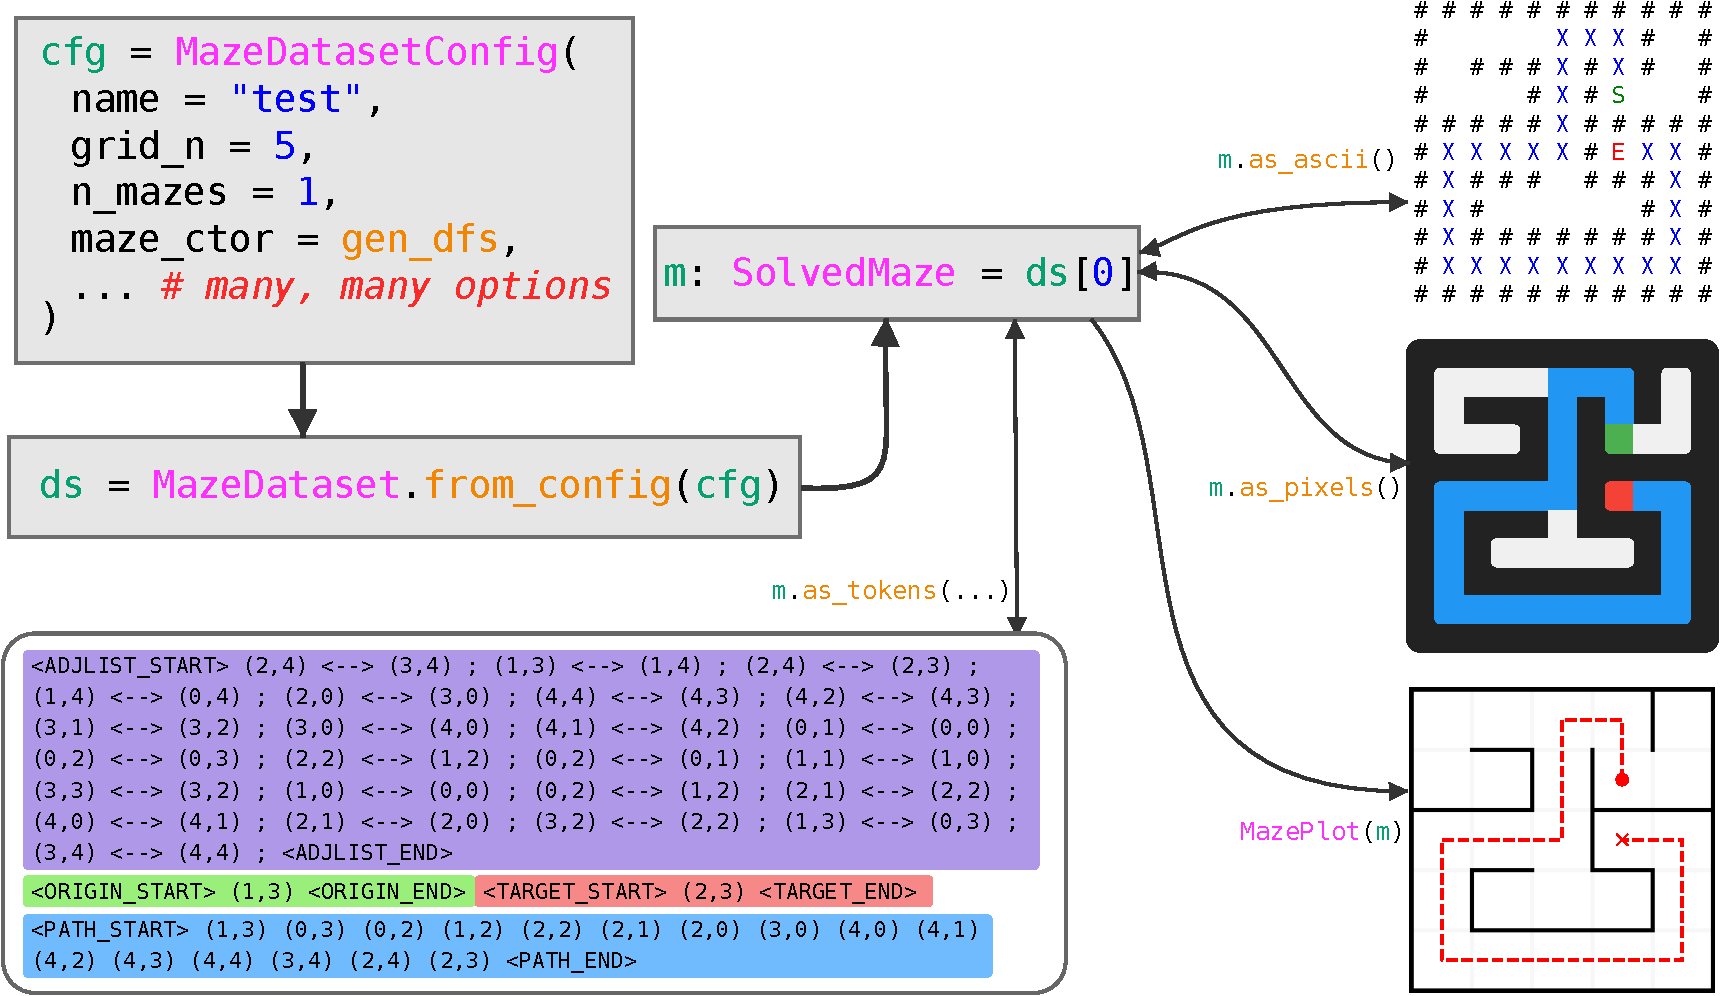
\includegraphics{docs/paper/diagram/diagram.pdf}%
};

\node[anchor=north west,
	hyperlink url={https://github.com},
	draw=blue, fill=blue!20, fill opacity=0.3,
	minimum width=2cm, minimum height=1cm]
	at ($(current page.north west)+(0,-1cm)$) {};

% Establish a coordinate system mapping the original SVG viewBox (1100x640)
% \begin{scope}[x={(img.south east)}, y={(img.north west)}]
	
% 	% 1. MazeDatasetConfig (for both "cfg" and "MazeDatasetConfig")
% 	\node[hyperlink url={https://understanding-search.github.io/maze-dataset/maze_dataset.html#MazeDatasetConfig},
% 			anchor=south west,
% 			draw=blue, fill=blue!20, fill opacity=0.3, line width=1pt,
% 			minimum width={(150-25)/1100*6in},
% 			minimum height={(60-30)/640*3.5in}]
% 		at ($(25/1100, {1 - 60/640})$) {};
	
% 	% 2. LatticeMazeGenerators.gen_dfs (the "gen_dfs" text)
% 	\node[hyperlink url={https://understanding-search.github.io/maze-dataset/maze_dataset.html#LatticeMazeGenerators.gen_dfs},
% 			anchor=south west,
% 			draw=blue, fill=blue!20, fill opacity=0.3, line width=1pt,
% 			minimum width={(150-45)/1100*6in},
% 			minimum height={(180-150)/640*3.5in}]
% 		at ($(45/1100, {1 - 180/640})$) {};
	
% 	% 3. MazeDataset (the "ds" and "MazeDataset" text)
% 	\node[hyperlink url={https://understanding-search.github.io/maze-dataset/maze_dataset.html#MazeDataset},
% 			anchor=south west,
% 			draw=blue, fill=blue!20, fill opacity=0.3, line width=1pt,
% 			minimum width={(150-25)/1100*6in},
% 			minimum height={(335-305)/640*3.5in}]
% 		at ($(25/1100, {1 - 335/640})$) {};
	
% 	% 4. MazeDataset.from_config (following MazeDataset on the same line)
% 	\node[hyperlink url={https://understanding-search.github.io/maze-dataset/maze_dataset.html#MazeDataset.from_config},
% 			anchor=south west,
% 			draw=blue, fill=blue!20, fill opacity=0.3, line width=1pt,
% 			minimum width={(300-150)/1100*6in},
% 			minimum height={(335-305)/640*3.5in}]
% 		at ($(150/1100, {1 - 335/640})$) {};
	
% 	% 5. SolvedMaze (the text starting at x≈424.6, y≈205)
% 	\node[hyperlink url={https://understanding-search.github.io/maze-dataset/maze_dataset.html#SolvedMaze},
% 			anchor=south west,
% 			draw=blue, fill=blue!20, fill opacity=0.3, line width=1pt,
% 			minimum width={(544.6-424.6)/1100*6in},  % 544.6 = 424.6+120
% 			minimum height={(205-165)/640*3.5in}]
% 		at ($(424.6/1100, {1 - 205/640})$) {};
	
% 	% 6. LatticeMaze.as_ascii (from x≈837.4, y≈125)
% 	\node[hyperlink url={https://understanding-search.github.io/maze-dataset/maze_dataset.html#LatticeMaze.as_ascii},
% 			anchor=south west,
% 			draw=blue, fill=blue!20, fill opacity=0.3, line width=1pt,
% 			minimum width={(937.4-837.4)/1100*6in},  % 937.4 = 837.4+100
% 			minimum height={(125-95)/640*3.5in}]
% 		at ($(837.4/1100, {1 - 125/640})$) {};
	
% 	% 7. LatticeMaze.as_pixels (from x≈836.1, y≈335)
% 	\node[hyperlink url={https://understanding-search.github.io/maze-dataset/maze_dataset.html#LatticeMaze.as_pixels},
% 			anchor=south west,
% 			draw=blue, fill=blue!20, fill opacity=0.3, line width=1pt,
% 			minimum width={(936.1-836.1)/1100*6in},  % 936.1 = 836.1+100
% 			minimum height={(335-305)/640*3.5in}]
% 		at ($(836.1/1100, {1 - 335/640})$) {};
	
% 	% 8. MazePlot (from x≈846.8, y≈555)
% 	\node[hyperlink url={https://understanding-search.github.io/maze-dataset/maze_dataset/plotting.html#MazePlot},
% 			anchor=south west,
% 			draw=blue, fill=blue!20, fill opacity=0.3, line width=1pt,
% 			minimum width={(966.8-846.8)/1100*6in},  % 966.8 = 846.8+120
% 			minimum height={(555-525)/640*3.5in}]
% 		at ($(846.8/1100, {1 - 555/640})$) {};
	
% 	% 9. LatticeMaze.as_tokens (from x≈571.1, y≈406)
% 	\node[hyperlink url={https://understanding-search.github.io/maze-dataset/maze_dataset.html#LatticeMaze.as_tokens},
% 			anchor=south west,
% 			draw=blue, fill=blue!20, fill opacity=0.3, line width=1pt,
% 			minimum width={(691.1-571.1)/1100*6in},  % 691.1 = 571.1+120
% 			minimum height={(406-376)/640*3.5in}]
% 		at ($(571.1/1100, {1 - 406/640})$) {};
	
% \end{scope}
\end{tikzpicture} 
  \end{minipage}
  \caption{
    Usage of maze-dataset. We create a \texttt{MazeDataset} from a \texttt{MazeDatasetConfig}. This contains \texttt{SolvedMaze} objects which can be converted to and from a variety of formats. Code in the image contains clickable links to \href{https://understanding-search.github.io/maze-dataset/maze_dataset.html}{documentation}. A variety of generated examples can be viewed \href{https://understanding-search.github.io/maze-dataset/examples/maze_examples.html}{here}.
  }
  \label{fig:diagram}
\end{figure}

\hypertarget{statement-of-need}{%
\section{Statement of Need}\label{statement-of-need}}

While maze generation itself is straightforward, the architectural
challenge comes from building a system supporting many algorithms with
configurable parameters, property filtering, and representation
transformation. This library aims to greatly streamline the process of
generating and working with datasets of mazes that can be described as
subgraphs of an \(n \times n\) lattice with boolean connections and,
optionally, start and end points that are nodes in the graph.
Furthermore, we place emphasis on a wide variety of possible text output
formats aimed at evaluating the spatial reasoning capabilities of Large
Language Models (LLMs) and other text-based transformer models.

For interpretability and behavioral research, algorithmic tasks offer
benefits by allowing systematic data generation and task decomposition,
as well as simplifying the process of circuit discovery
(\protect\hyperlink{ref-interpretability-survery}{Räuker et al., 2023}).
Although mazes are well suited for these investigations, we found that
existing maze generation packages
(\protect\hyperlink{ref-cobbe2019procgen}{Cobbe et al., 2019};
\protect\hyperlink{ref-gh_Ehsan_2022}{Ehsan, 2022};
\protect\hyperlink{ref-harriesMazeExplorerCustomisable3D2019}{Harries et
al., n.d.}; \protect\hyperlink{ref-gh_Nemeth_2019}{Németh, 2019};
\protect\hyperlink{ref-easy_to_hard}{Schwarzschild, Borgnia, Gupta,
Bansal, et al., 2021}) lack support for transforming between multiple
representations and provide limited control over the maze generation
process.

\hypertarget{related-works}{%
\subsection{Related Works}\label{related-works}}

A multitude of public and open-source software packages exist for
generating mazes (\protect\hyperlink{ref-gh_Ehsan_2022}{Ehsan, 2022};
\protect\hyperlink{ref-gh_Nemeth_2019}{Németh, 2019};
\protect\hyperlink{ref-easy_to_hard}{Schwarzschild, Borgnia, Gupta,
Bansal, et al., 2021}). However, nearly all of these packages produce
mazes represented as rasterized images or other visual formats rather
than the underlying graph structure, and this makes it difficult to work
with these datasets.

\begin{itemize}
\item
  Most prior works provide mazes in visual or raster formats, and we
  provide a variety of similar output formats:

  \begin{itemize}
  \tightlist
  \item
    \href{https://understanding-search.github.io/maze-dataset/maze_dataset/dataset/rasterized.html\#RasterizedMazeDataset}{\texttt{RasterizedMazeDataset}},
    utilizing
    \href{https://understanding-search.github.io/maze-dataset/maze_dataset.html\#LatticeMaze.as_pixels}{\texttt{as\_pixels()}},
    which can exactly mimic the outputs provided in
    \texttt{easy-to-hard-data}(\protect\hyperlink{ref-easy_to_hard}{Schwarzschild,
    Borgnia, Gupta, Bansal, et al., 2021}) and can be configured to be
    similar to the outputs of Németh
    (\protect\hyperlink{ref-gh_Nemeth_2019}{2019})
  \item
    \href{https://understanding-search.github.io/maze-dataset/maze_dataset.html\#LatticeMaze.as_ascii}{\texttt{as\_ascii()}}
    provides a format similar to
    (\protect\hyperlink{ref-gh-oppenheimj2018maze}{Oppenheim, 2018};
    \protect\hyperlink{ref-eval-gpt-visual}{Singla, 2023})
  \item
    \href{https://understanding-search.github.io/maze-dataset/maze_dataset/plotting.html\#MazePlot}{\texttt{MazePlot}}
    provides a feature-rich plotting utility with support for multiple
    paths, heatmaps over positions, and more. This is similar to the
    outputs of (\protect\hyperlink{ref-mazegenerator-net}{Alance AB,
    2019}; \protect\hyperlink{ref-gh_Ehsan_2022}{Ehsan, 2022};
    \protect\hyperlink{ref-mathematica-maze}{Guo et al., 2011};
    \protect\hyperlink{ref-mdl-suite}{Nag, 2020})
  \end{itemize}
\item
  The text format provided by
  \href{https://understanding-search.github.io/maze-dataset/maze_dataset.html\#MazeDataset.as_tokens}{\texttt{SolvedMaze(...).as\_tokens()}}
  is similar to that of (\protect\hyperlink{ref-eval-LLM-graphs}{Liu \&
  Wu, 2023}), but provides over 5.8 million unique formats for
  converting mazes to a text stream, detailed in
  \hyperref[sec:tokenized-output-formats]{section: \textit{\nameref{sec:tokenized-output-formats}}}.
\item
  For rigorous investigations of the response of a model to various
  distributional shifts, preserving metadata about the generation
  algorithm with the dataset itself is essential. To this end, our
  package efficiently stores the dataset along with its metadata in a
  single human-readable file (\protect\hyperlink{ref-zanj}{M.
  Ivanitskiy, n.d.}). As far as we are aware, no existing packages do
  this reliably.
\item
  Storing mazes as images is not only difficult to work with, but also
  inefficient. We use a highly efficient method detailed in
  \hyperref[sec:implementation]{section: \textit{\nameref{sec:implementation}}}.
\item
  Our package is easily installable with source code freely available.
  It is extensively tested, type hinted, benchmarked, and documented.
  Many other maze generation packages lack this level of rigor and
  scope, and some (\protect\hyperlink{ref-ayaz2008maze}{Ayaz et al.,
  2008}) appear to simply no longer be accessible.
\end{itemize}

\hypertarget{features}{%
\section{Features}\label{features}}

We direct readers to our
\href{https://understanding-search.github.io/maze-dataset/examples/maze_examples.html}{examples},
\href{https://understanding-search.github.io/maze-dataset/maze_dataset.html}{docs},
and
\href{https://understanding-search.github.io/maze-dataset/notebooks/}{notebooks}
for more information.

\hypertarget{generation}{%
\subsection{Generation and Basic Usage}\label{generation}}

Our package can be installed from
\href{https://pypi.org/project/maze-dataset/}{PyPi} via
\texttt{pip\ install\ maze-dataset}, or directly from the
\href{https://github.com/understanding-search/maze-dataset}{git
repository} (\protect\hyperlink{ref-maze-dataset-github}{Michael I.
Ivanitskiy et al., 2023a}).

To create a dataset, we first create a
\href{https://understanding-search.github.io/maze-dataset/maze_dataset.html\#MazeDatasetConfig}{\texttt{MazeDatasetConfig}}
configuration object, which specifies the seed, number, and size of
mazes, as well as the generation algorithm and its corresponding
parameters. This object is passed to a
\href{https://understanding-search.github.io/maze-dataset/maze_dataset.html\#MazeDataset}{\texttt{MazeDataset}}
class to create a dataset. Crucially, this
\href{https://understanding-search.github.io/maze-dataset/maze_dataset.html\#MazeDataset}{\texttt{MazeDataset}}
mimics the interface of a PyTorch
(\protect\hyperlink{ref-pytorch}{Paszke et al., 2019})
\href{https://pytorch.org/docs/stable/data.html}{\texttt{Dataset}}, and
can thus be easily incorporated into existing data pre-processing and
training pipelines, e.g., through the use of a \texttt{DataLoader}
class.

\begin{Shaded}
\begin{Highlighting}[]
\ImportTok{from}\NormalTok{ maze\_dataset }\ImportTok{import}\NormalTok{ (}
\NormalTok{  MazeDataset, MazeDatasetConfig, LatticeMazeGenerators}
\NormalTok{)}
\CommentTok{\# create a config}
\NormalTok{cfg: MazeDatasetConfig }\OperatorTok{=}\NormalTok{ MazeDatasetConfig(}
\NormalTok{    name}\OperatorTok{=}\StringTok{"example"}\NormalTok{, }\CommentTok{\# names need not be unique}
\NormalTok{    grid\_n}\OperatorTok{=}\DecValTok{3}\NormalTok{,   }\CommentTok{\# size of the maze}
\NormalTok{    n\_mazes}\OperatorTok{=}\DecValTok{32}\NormalTok{, }\CommentTok{\# number of mazes in the dataset}
\NormalTok{    maze\_ctor}\OperatorTok{=}\NormalTok{LatticeMazeGenerators.gen\_dfs, }\CommentTok{\# many algorithms available}
    \CommentTok{\# (optional) algorithm{-}specific parameters}
\NormalTok{    maze\_ctor\_kwargs}\OperatorTok{=}\NormalTok{\{}\StringTok{"do\_forks"}\NormalTok{: }\VariableTok{True}\NormalTok{, ...\}, }
    \CommentTok{\# (optional) many options for restricting start/end points}
\NormalTok{    endpoint\_kwargs}\OperatorTok{=}\NormalTok{\{}\StringTok{"deadend\_start"}\NormalTok{: }\VariableTok{True}\NormalTok{, ...\},}
\NormalTok{)}
\CommentTok{\# create a dataset}
\NormalTok{dataset: MazeDataset }\OperatorTok{=}\NormalTok{ MazeDataset.from\_config(}
\NormalTok{  cfg, }\CommentTok{\# pass the config}
\NormalTok{  ..., }\CommentTok{\# other options for disk loading, parallelization, etc.}
\NormalTok{)}
\end{Highlighting}
\end{Shaded}

When initializing a dataset, options which do not affect the mazes
themselves can be specified through the
\href{https://understanding-search.github.io/maze-dataset/maze_dataset.html\#MazeDataset.from_config}{\texttt{from\_config()}}
factory method as necessary. These options allow for saving/loading
existing datasets instead of re-generating, parallelization options for
generation, and more. Available maze generation algorithms are static
methods of the
\href{https://understanding-search.github.io/maze-dataset/maze_dataset.html\#LatticeMazeGenerators}{\texttt{LatticeMazeGenerators}}
namespace class and include generation algorithms based on randomized
depth-first search, Wilson's algorithm
(\protect\hyperlink{ref-wilson}{Wilson, 1996}), percolation
(\protect\hyperlink{ref-percolation}{Duminil-Copin, 2017};
\protect\hyperlink{ref-percolation-clustersize}{Fisher \& Essam, 2004}),
Kruskal's algorithm
(\protect\hyperlink{ref-kruskal1956shortest}{Kruskal, 1956}), and
others.

Furthermore, a dataset of mazes can be filtered to satisfy certain
properties. Custom filters can be specified, and some filters are
included in
\href{https://understanding-search.github.io/maze-dataset/maze_dataset/dataset/filters.html\#MazeDatasetFilters}{\texttt{MazeDatasetFilters}}.
For example, we can require a minimum path length of three steps from
the origin to the target:

\begin{Shaded}
\begin{Highlighting}[]
\NormalTok{dataset\_filtered: MazeDataset }\OperatorTok{=}\NormalTok{ dataset.filter\_by.path\_length(min\_length}\OperatorTok{=}\DecValTok{3}\NormalTok{)}
\end{Highlighting}
\end{Shaded}

All implemented maze generation algorithms are stochastic by nature. For
reproducibility, the \texttt{seed} parameter of
\href{https://understanding-search.github.io/maze-dataset/maze_dataset.html\#MazeDatasetConfig}{\texttt{MazeDatasetConfig}}
may be set. In practice, using provided deduplication filters, we find
that exact duplicate mazes are generated very infrequently, even when
generating very large datasets.

For use cases where mazes of different sizes, generation algorithms, or
other parameter variations are required, we provide the
\href{https://understanding-search.github.io/maze-dataset/maze_dataset/dataset/collected_dataset.html\#MazeDatasetCollection}{\texttt{MazeDatasetCollection}}
class, which allows for creating a single iterable dataset from multiple
independent configurations.

\hypertarget{visual-output-formats}{%
\subsection{Visual Output Formats}\label{visual-output-formats}}

Internally, mazes are
\href{https://understanding-search.github.io/maze-dataset/maze_dataset.html\#SolvedMaze}{\texttt{SolvedMaze}}
objects, which have path information and a tensor optimized for storing
sub-graphs of a lattice. These objects can be converted to and from
several formats to maximize their utility in different contexts.

\begin{figure}[H]
  \centering
  \begin{tabular}{p{1.5in} p{1.5in} p{1.5in}} 
    \hline \\[.5em]
    % algorithms
    \href{https://understanding-search.github.io/maze-dataset/maze_dataset.html\#LatticeMaze.as_ascii}{\texttt{as\_ascii()}}
    & \href{https://understanding-search.github.io/maze-dataset/maze_dataset.html\#LatticeMaze.as_pixels}{\texttt{as\_pixels()}}
    & \href{https://understanding-search.github.io/maze-dataset/maze_dataset/plotting.html\#MazePlot}{\texttt{MazePlot()}} \\[.5em]
    % descriptions
      Simple text format for displaying mazes, useful for debugging in a terminal environment.
      & \texttt{numpy} array of \texttt{dtype=uint8} and shape \texttt{(height, width, 3)}. The last dimension is RGB color.
      & feature-rich plotting utility with support for multiple paths, heatmaps over positions, and more. \\[1em]
    \hline \\
    % examples
      \multicolumn{1}{c}{\begin{minipage}[b]{1.6in}
        \setlength{\baselineskip}{0.9em}
        {
% \footnotesize
\ttfamily
\setlength{\tabcolsep}{0.3em}
\renewcommand{\arraystretch}{0.75}
\begin{tabular}{ccccccccccc}
\# & \# & \# & \# & \# & \# & \# & \# & \# & \# & \# \\
\# &   &   &   &   & \textcolor{blue}{X} & \textcolor{blue}{X} & \textcolor{blue}{X} & \# &  & \# \\
\# &   & \# & \# & \# & \textcolor{blue}{X} & \# & \textcolor{blue}{X} & \# &   & \# \\
\# &   &   &   & \# & \textcolor{blue}{X} & \# & \textcolor{green}{S} &   &   & \# \\
\# & \# & \# & \# & \# & \textcolor{b			lue}{X} & \# & \# & \# & \# & \# \\
\# & \textcolor{blue}{X} & \textcolor{blue}{X} & \textcolor{blue}{X} & \textcolor{blue}{X} & \textcolor{blue}{X} & \# & \textcolor{red}{E} & \textcolor{blue}{X} & \textcolor{blue}{X} & \# \\
\# & \textcolor{blue}{X} & \# & \# & \# &   & \# & \# & \# & \textcolor{blue}{X} & \# \\
\# & \textcolor{blue}{X} & \# &   &   &   &   &   & \# & \textcolor{blue}{X} & \# \\
\# & \textcolor{blue}{X} & \# & \# & \# & \# & \# & \# & \# & \textcolor{blue}{X} & \# \\
\# & \textcolor{blue}{X} & \textcolor{blue}{X} & \textcolor{blue}{X} & \textcolor{blue}{X} & \textcolor{blue}{X} & \textcolor{blue}{X} & \textcolor{blue}{X} & \textcolor{blue}{X} & \textcolor{blue}{X} & \# \\
\# & \# & \# & \# & \# & \# & \# & \# & \# & \# & \#
\end{tabular}
} 
      \end{minipage}}
      & \multicolumn{1}{c}{
        
\includegraphics[width=0.25\textwidth]{figures/outputs-pixels.pdf}
      }
      & \multicolumn{1}{c}{
        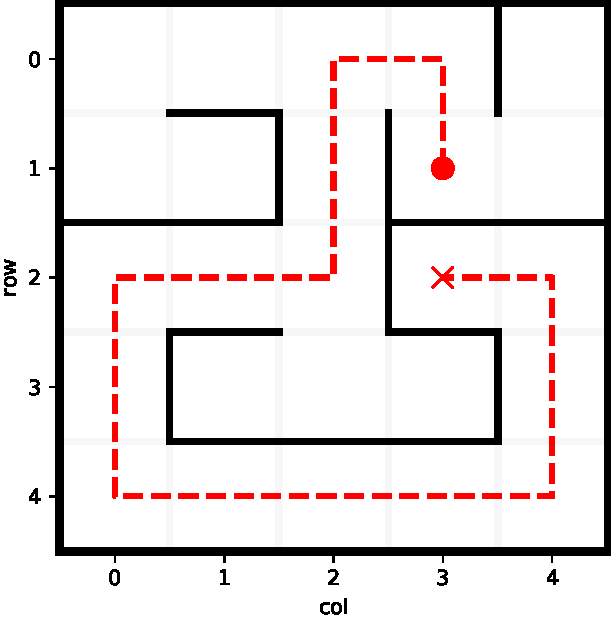
\includegraphics[width=0.27\textwidth, trim={0 0.8cm -.3cm, -.5cm}, clip]{figures/outputs-mazeplot.pdf}
      } \\[1em]
    
    \hline \\
  \end{tabular}
  \caption{Various output formats. Top row (left to right): ASCII diagram, rasterized pixel grid, and advanced display tool.}
  \label{fig:output-fmts}
\end{figure}

In previous work, maze tasks have been used with Recurrent Convolutional
Neural Network (RCNN) derived architectures
(\protect\hyperlink{ref-deepthinking}{Schwarzschild, Borgnia, Gupta,
Huang, et al., 2021}). To facilitate the use of our package in this
context, we replicate the format of
(\protect\hyperlink{ref-easy_to_hard}{Schwarzschild, Borgnia, Gupta,
Bansal, et al., 2021}) and provide the
\href{https://understanding-search.github.io/maze-dataset/maze_dataset/dataset/rasterized.html\#RasterizedMazeDataset}{\texttt{RasterizedMazeDataset}}
class which returns rasterized pairs of (input, target) mazes as shown
in \autoref{fig:e2h-raster} below.

\begin{figure}
\hypertarget{fig:e2h-raster}{%
\centering

\includegraphics[width=0.3\textwidth,height=\textheight]{figures/maze-raster-input-target.pdf}
\caption{Input is the rasterized maze without the path marked (left),
and provide as a target the maze with all but the correct path removed
(right). Configuration options exist to adjust whether endpoints are
included and if empty cells should be filled in.}\label{fig:e2h-raster}
}
\end{figure}

\hypertarget{sec:tokenized-output-formats}{%
\subsection{Tokenized Output
Formats}\label{sec:tokenized-output-formats}}

Autoregressive transformer models can be quite sensitive to the exact
format of input data, and may even use delimiter tokens to perform
reasoning steps (\protect\hyperlink{ref-pfau2024dotbydot}{Pfau et al.,
2024}; \protect\hyperlink{ref-spies2024causalworldmodels}{Spies et al.,
2024}). To facilitate systematic investigation of the effects of
different representations of data on text model performance, we provide
a variety of tokenized text output formats.

We convert mazes to token sequences in two steps. First, the maze is
stringified using
\href{https://understanding-search.github.io/maze-dataset/maze_dataset.html\#MazeDataset.as_tokens}{\texttt{as\_tokens()}}.
The
\href{https://understanding-search.github.io/maze-dataset/maze_dataset/tokenization.html\#MazeTokenizerModular}{\texttt{MazeTokenizerModular}}
class provides a powerful interface for configuring maze stringification
behavior. Second, the sequence of strings is tokenized into integers
using \texttt{encode()}. Tokenization uses a fixed vocabulary for
simplicity. Mazes up to \(50 \times 50\) are supported when using a
unique token for each position, and up to \(128 \times 128\) are
supported when positions in the maze are represented as a pair of
coordinates.

There are many algorithms by which one might tokenize a 2D maze into a
1D format usable by autoregressive text models. Training multiple models
on the encodings output from each of these algorithms may produce very
different internal representations, learned solution algorithms, and
levels of performance. To allow exploration of how different maze
tokenization algorithms affect these models, the
\href{https://understanding-search.github.io/maze-dataset/maze_dataset/tokenization.html\#MazeTokenizerModular}{\texttt{MazeTokenizerModular}}
class contains a rich set of options to customize how mazes are
stringified. This class contains 19 discrete parameters, resulting in
over 5.8 million unique tokenizers. There are 6 additional parameters
available whose functionality is not verified via automated testing, but
further expand the the number of tokenizers by a factor of \(44/3\) to
86 million.

All output sequences consist of four token regions representing
different features of the maze; an example output sequence is shown in
\autoref{fig:token-regions}.

\begin{figure} 
  \centering
  \begin{minipage}{5in}
    \footnotesize
    % could not figure out how to make lines break a colorbox, so that's why these line breaks are manual
\colorbox[RGB]{ 217,210,233 }{ \texttt{ <ADJLIST\_START> (0,0) <--> (1,0) ; (2,0) <--> (3,0) ; (4,1) <--> (4,0) ; (2,0) <--> (2,1) ; }} 
\colorbox[RGB]{ 217,210,233 }{ \texttt{ (1,0) <--> (1,1) ; (3,4) <--> (2,4) ; (4,2) <--> (4,3) ; (0,0) <--> (0,1) ; (0,3) <--> (0,2) ; }}
\colorbox[RGB]{ 217,210,233 }{ \texttt{ (4,4) <--> (3,4) ; (4,3) <--> (4,4) ; (4,1) <--> (4,2) ; (2,1) <--> (2,2) ; (1,4) <--> (0,4) ; }}
\colorbox[RGB]{ 217,210,233 }{ \texttt{ (1,2) <--> (0,2) ; (2,4) <--> (2,3) ; (4,0) <--> (3,0) ; (2,2) <--> (3,2) ; (1,2) <--> (2,2) ; }} 
\colorbox[RGB]{ 217,210,233 }{ \texttt{ (1,3) <--> (0,3) ; (3,2) <--> (3,3) ; (0,2) <--> (0,1) ; (3,1) <--> (3,2) ; (1,3) <--> (1,4) ; }}
\colorbox[RGB]{ 217,210,233 }{ \texttt{ <ADJLIST\_END> } } \colorbox[RGB]{ 217,234,211 }{ \texttt{ <ORIGIN\_START> (1,3) <ORIGIN\_END> } } 
\colorbox[RGB]{ 234,209,220 }{ \texttt{ <TARGET\_START> (2,3) <TARGET\_END> } } 
\colorbox[RGB]{ 207,226,243 }{ \texttt{ <PATH\_START> (1,3) (0,3) (0,2) (1,2) (2,2) (2,1) (2,0) (3,0) (4,0) (4,1) (4,2) (4,3) (4,4) }}
\colorbox[RGB]{ 207,226,243 }{ \texttt{ (3,4) (2,4) (2,3) <PATH\_END> } } \\
  \end{minipage}
  \caption{
    Example text output format with token regions highlighted.
    \colorbox[RGB]{ 217,210,233 }{Adjacency list}: text representation of the graph,
    \colorbox[RGB]{ 217,234,211 }{Origin}: starting coordinate,
    \colorbox[RGB]{ 234,209,220 }{Target}: ending coordinate,
    \colorbox[RGB]{ 207,226,243 }{Path}: maze solution sequence
  }
  \label{fig:token-regions}
\end{figure}

Each
\href{https://understanding-search.github.io/maze-dataset/maze_dataset/tokenization.html\#MazeTokenizerModular}{\texttt{MazeTokenizerModular}}
is constructed from a set of several
\href{https://understanding-search.github.io/maze-dataset/maze_dataset/tokenization.html\#_TokenizerElement}{\texttt{\_TokenizerElement}}
objects, each of which specifies how different token regions or other
elements of the stringification are produced.

\begin{figure}
    \centering
    \begin{tikzpicture}[
S1/.style={rectangle, rounded corners, draw=red!60, fill=red!5, very thick,
minimum size=5mm},
S2/.style={rectangle, rounded corners, draw=blue!60, fill=blue!5, very thick, minimum size=5mm},
]
	\node[
	S1, 
	minimum height=0.42\textwidth, 
	minimum width=0.65\textwidth, 
	text depth=0.42\textwidth,
	] (MTM) 
	{\texttt{MazeTokenizerModular}};
	\node[
	S2, 
	minimum height=0.37\textwidth, 
	minimum width=0.62\textwidth, 
	text depth=0.37\textwidth,
	] (PS) 
	at ($ (MTM) + (0,-0.01\textwidth) $)
	{\texttt{\_PromptSequencer}};
	\node[
	S1, 
	% minimum height=0.1\textwidth, 
	minimum width=0.59\textwidth, 
	% text depth=0.1\textwidth,
	] (CT) 
	at ($ (PS) + (0,0.135\textwidth) $)
	{\texttt{\_CoordTokenizer}};
	\node[
	S1, 
	minimum height=0.07\textwidth, 
	minimum width=0.59\textwidth, 
	text depth=0.05\textwidth,
	% fill={rgb:red,217;green,210;blue,233}, % TODO: get colors to match the ones in fig:output-tokenized
	] (Adj) 
	at ($ (CT) + (0,-0.07\textwidth) $)
	{\texttt{\_AdjListTokenizer}};
	\node[
	S1, 
	% minimum height=0.1\textwidth, 
	minimum width=0.59\textwidth, 
	% text depth=0.1\textwidth,
	] (Target) 
	at ($ (Adj) + (0,-0.07\textwidth) $)
	{\texttt{\_TargetTokenizer}};
	\node[
	S1, 
	minimum height=0.14\textwidth, 
	minimum width=0.59\textwidth, 
	text depth=0.12\textwidth,
	] (Path) 
	at ($ (Target) + (0,-0.105\textwidth) $)
	{\texttt{\_PathTokenizer}};
	\node[
	S2, 
	% minimum height=0.1\textwidth, 
	minimum width=0.17\textwidth, 
	% text depth=0.1\textwidth,
	] (ESubset) 
	at ($ (Adj) + (-0.19\textwidth,-0.01\textwidth) $)
	{\texttt{\_EdgeSubset}};
	\node[
	S2, 
	% minimum height=0.1\textwidth, 
	minimum width=0.17\textwidth, 
	% text depth=0.1\textwidth,
	] (EGrouping) 
	at ($ (Adj) + (-0.0\textwidth,-0.01\textwidth) $)
	{\texttt{\_EdgeGrouping}};
	\node[
	S2, 
	% minimum height=0.1\textwidth, 
	minimum width=0.17\textwidth, 
	% text depth=0.1\textwidth,
	] (EPermuter) 
	at ($ (Adj) + (0.19\textwidth,-0.01\textwidth) $)
	{\texttt{\_EdgePermuter}};
	
	\node[
	S2, 
	minimum height=0.1\textwidth, 
	minimum width=0.2\textwidth, 
	% text depth=0.1\textwidth,
	] (StepSize) 
	at ($ (Path) + (-0.105\textwidth,-0.01\textwidth) $)
	{\texttt{\_StepSize}};
	\node[
	S2, 
	% minimum height=0.1\textwidth, 
	minimum width=0.2\textwidth, 
	% text depth=0.1\textwidth,
	] (StepTok1) 
	at ($ (Path) + (0.105\textwidth,0.025\textwidth) $)
	{\texttt{\_StepTokenizer}};
	\node[
	S2, 
	% minimum height=0.1\textwidth, 
	minimum width=0.2\textwidth, 
	% text depth=0.1\textwidth,
	] (StepTok2) 
	at ($ (StepTok1) + (0,-0.04\textwidth) $)
	{\texttt{\_StepTokenizer}};
	\node
	at ($ (StepTok2) + (0,-0.03\textwidth) $)
	{$\vdots$};
\end{tikzpicture}
    \caption{Nested internal structure of \texttt{\_TokenizerElement} objects inside a typical \texttt{MazeTokenizerModular}.}
\end{figure}

The tokenizer architecture is purposefully designed such that adding and
testing a wide variety of new tokenization algorithms is fast and
minimizes disturbances to functioning code. This is enabled by the
modular architecture and the automatic inclusion of any new tokenizers
in integration tests. To create a new variety of tokenizer, developers
forking the library may simply create their own
\href{https://understanding-search.github.io/maze-dataset/maze_dataset/tokenization.html\#_TokenizerElement}{\texttt{\_TokenizerElement}}
subclass and implement the abstract methods. If the behavior change is
sufficiently small, simply adding a parameter to an existing
\href{https://understanding-search.github.io/maze-dataset/maze_dataset/tokenization.html\#_TokenizerElement}{\texttt{\_TokenizerElement}}
subclass and updating its implementation will suffice.

The breadth of tokenizers is also easily scaled in the opposite
direction. Due to the exponential scaling of parameter combinations,
adding a small number of new features can significantly slow certain
procedures which rely on constructing all possible tokenizers, such as
integration tests. If any existing subclass contains features which
aren't needed, a developer tool decorator
\href{https://understanding-search.github.io/maze-dataset/maze_dataset/tokenization/modular/element_base.html\#mark_as_unsupported}{\texttt{@mark\_as\_unsupported}}
is provided which can be applied to the unneeded
\href{https://understanding-search.github.io/maze-dataset/maze_dataset/tokenization.html\#_TokenizerElement}{\texttt{\_TokenizerElement}}
subclasses to prune those features and compact the available space of
tokenizers.

\hypertarget{benchmarks}{%
\subsection{Benchmarks of Generation Speed}\label{benchmarks}}

We provide approximate benchmarks for relative generation time across
various algorithms, parameter choices, maze sizes, and dataset sizes in
\autoref{tab:benchmarks} and \autoref{fig:benchmarks}. Experiments were
performed on a
\href{https://docs.github.com/en/actions/using-github-hosted-runners/using-github-hosted-runners/about-github-hosted-runners#standard-github-hosted-runners-for-public-repositories}{standard GitHub runner}
without parallelism.

\begin{table}[H]
\centering
\begin{tabular}{|ll|r|rrr|}
  \hline
  maze\_ctor
          & keyword args           & all sizes 
                                              & \shortstack{small \\ $g \leq 10$} 
                                                         & \shortstack{medium \\ $g \in (10, 32]$} 
                                                                    & \shortstack{large \\ $g > 32$} \\
  \hline\hline
  \href{https://understanding-search.github.io/maze-dataset/maze_dataset.html\#LatticeMazeGenerators.gen_dfs}{dfs}
          &                        &   28.0   &    2.8   &   20.3   &  131.8   \\
  \href{https://understanding-search.github.io/maze-dataset/maze_dataset.html\#LatticeMazeGenerators.gen_dfs}{dfs}
          & accessible\_cells=20   &    2.3   &    2.2   &    2.4   &    2.2   \\
  \href{https://understanding-search.github.io/maze-dataset/maze_dataset.html\#LatticeMazeGenerators.gen_dfs}{dfs}
          & do\_forks=False        &    2.7   &    2.2   &    3.1   &    3.5   \\
  \href{https://understanding-search.github.io/maze-dataset/maze_dataset.html\#LatticeMazeGenerators.gen_dfs}{dfs}
          & max\_tree\_depth=0.5   &    2.5   &    2.0   &    2.7   &    4.0   \\
  \href{https://understanding-search.github.io/maze-dataset/maze_dataset.html\#LatticeMazeGenerators.gen_dfs_percolation}{dfs\_percolation}
          & p=0.1                  &   43.9   &    2.8   &   33.9   &  208.0   \\
  \href{https://understanding-search.github.io/maze-dataset/maze_dataset.html\#LatticeMazeGenerators.gen_dfs_percolation}{dfs\_percolation}
          & p=0.4                  &   48.7   &    3.0   &   36.5   &  233.5   \\
  \href{https://understanding-search.github.io/maze-dataset/maze_dataset.html\#LatticeMazeGenerators.gen_kruskal}{kruskal}
          &                        &   12.8   &    1.9   &   10.3   &   55.8   \\
  \href{https://understanding-search.github.io/maze-dataset/maze_dataset.html\#LatticeMazeGenerators.gen_percolation}{percolation}
          & p=1.0                  &   50.2   &    2.6   &   37.2   &  242.5   \\
  \href{https://understanding-search.github.io/maze-dataset/maze_dataset.html\#LatticeMazeGenerators.gen_recursive_division}{recursive\_div}
          &                        &   10.2   &    1.7   &    8.9   &   42.1   \\
  \href{https://understanding-search.github.io/maze-dataset/maze_dataset.html\#LatticeMazeGenerators.gen_wilson}{wilson}
          &                        &  676.5   &    7.8   &  188.6   & 3992.6   \\
  \hline\hline
  mean
          &                        &  559.9   &   13.0   &  223.5   & 3146.9   \\
  median
          &                        &   11.1   &    6.5   &   32.9   &  302.7   \\
  \hline
\end{tabular}
\caption{Generation times for various algorithms and maze sizes.}
\label{tab:benchmarks}
\end{table}

\begin{figure}
\hypertarget{fig:benchmarks}{%
\centering
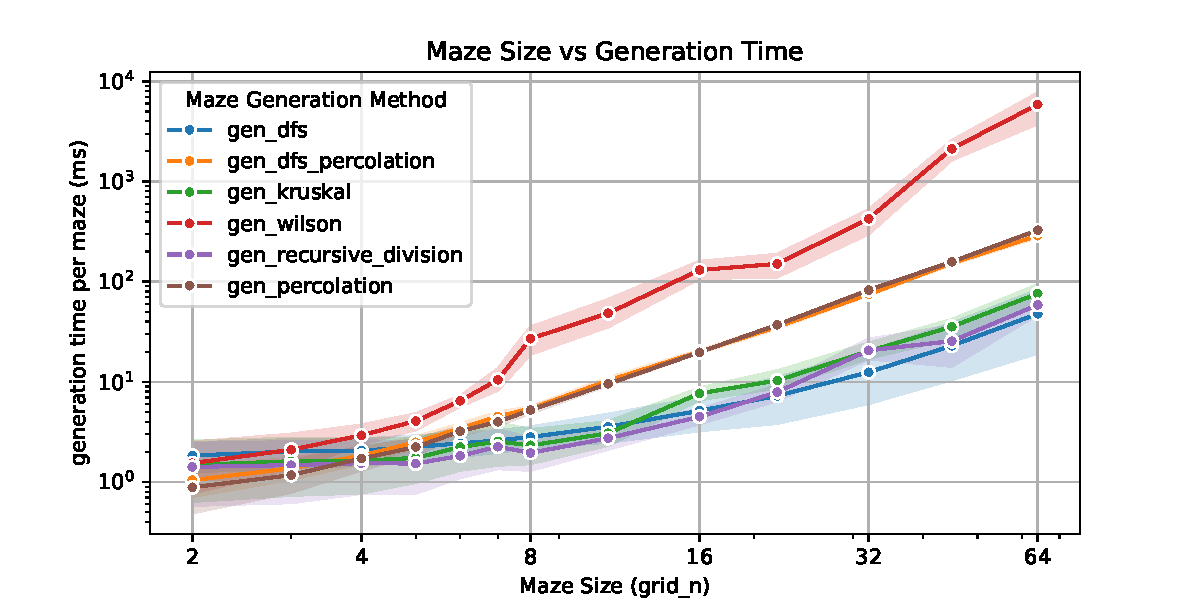
\includegraphics[width=0.95\textwidth,height=\textheight]{figures/benchmarks/gridsize-vs-gentime.pdf}
\caption{Plot of maze generation time. Generation time scales
exponentially with maze size for all algorithms. Generation time per
maze does not depend on the number of mazes being generated, and there
is minimal overhead to initializing the generation process for a small
dataset. Wilson's algorithm is notably less efficient than others and
has high variance. Note that values are averaged across all parameter
sets for that algorithm. More information can be found on the
\href{https://understanding-search.github.io/maze-dataset/benchmarks/}{benchmarks
page}.}\label{fig:benchmarks}
}
\end{figure}

\hypertarget{sec:success-rate-estimation}{%
\subsection{Success Rate Estimation}\label{sec:success-rate-estimation}}

In order to replicate the exact dataset distribution of
(\protect\hyperlink{ref-easy_to_hard}{Schwarzschild, Borgnia, Gupta,
Bansal, et al., 2021}), the parameter
\href{https://understanding-search.github.io/maze-dataset/maze_dataset/dataset/maze_dataset_config.html\#MazeDatasetConfig.endpoint_kwargs}{\texttt{MazeDatasetConfig.endpoint\_kwargs:}}
\href{https://understanding-search.github.io/maze-dataset/maze_dataset/dataset/maze_dataset_config.html\#EndpointKwargsType}{\texttt{EndpointKwargsType}}
allows for additional constraints such as enforcing that the start or
end point be in a ``dead end'' with only one accessible neighbor cell.
However, combining these constraints with cyclic mazes (such as those
generated with percolation), as was required for the work in
(\protect\hyperlink{ref-knutson2024logicalextrapolation}{Knutson et al.,
2024}), can lead to an absence of valid start and end points. Placing
theoretical bounds on this success rate is difficult, as it depends on
the exact maze generation algorithm and parameters used. To deal with
this, our package provides a way to estimate the success rate of a given
configuration using a symbolic regression model trained with PySR
(\protect\hyperlink{ref-pysr}{Cranmer, 2023}). More details on this can
be found in
\href{https://understanding-search.github.io/maze-dataset/notebooks/estimate_dataset_fractions.html}{\texttt{estimate\_dataset\_fractions.ipynb}}.
Using the estimation algorithm simply requires the user to call
\href{https://understanding-search.github.io/maze-dataset/maze_dataset.html\#MazeDatasetConfig.success_fraction_compensate}{\texttt{cfg\_new:\ MazeDatasetConfig\ =\ cfg.success\_fraction\_compensate()}},
providing their initial \texttt{cfg} and then using the returned
\texttt{cfg\_new} in its place.

\hypertarget{success-rate-estimation-algorithm}{%
\subsubsection{Success Rate Estimation
Algorithm}\label{success-rate-estimation-algorithm}}

The base function learned by symbolic regression privdes limited insight
and may be subject to change. It is defined as
\href{https://understanding-search.github.io/maze-dataset/maze_dataset/dataset/success_predict_math.html\#cfg_success_predict_fn}{\texttt{cfg\_success\_predict\_fn}},
and takes a 5 dimensional float vector created by
\texttt{MazeDatasetConfig.\_to\_ps\_array()} which represents the 0)
percolation value 1) grid size 2) endpoint deadend configuration 3)
endpoint uniqueness 4) categorical generation function index.

However, the outputs of this function are not directly usable due to
minor divergences at the endpoints with respect to the percolation
probability \(p\). Since we know that maze success is either guaranteed
or impossible for \(p=0\) and \(p=1\), we define the
\href{https://understanding-search.github.io/maze-dataset/maze_dataset/dataset/success_predict_math.html\#soft_step}{\texttt{soft\_step}}
function to nudge the raw output of the symbolic regression. This
function is defined with the following components:

shifted sigmoid \(\sigma_s\), amplitude scaling \(A\), and \(h\)
function given by \[
  \sigma_s(x) = (1 + e^{-10^3 \cdot (x-0.5)})^{-1}
  \qquad A(q,a,w) = w \cdot (1 - |2q-1|^a)
\] \[
  h(q,a) = q \cdot (1 - |2q-1|^a) \cdot (1-\sigma_s(q)) + (1-(1-q) \cdot (1 - |2(1-q)-1|^a)) \cdot \sigma_s(q)
\]

We combine these to get the
\href{https://understanding-search.github.io/maze-dataset/maze_dataset/dataset/success_predict_math.html\#soft_step}{\texttt{soft\_step}}
function, which is identity-like for \(p \approx 0.5\), and pushes
pushes \(x\) to extremes otherwise. \[
  \text{soft\_step}(x, p, \alpha, w) = h(x, A(p, \alpha, w))
\]

Finally, we define \[
  \text{cfg\_success\_predict\_fn}(\mathbf{x}) = \text{soft\_step}(\text{raw\_val}, x_0, 5, 10)
\]

where \texttt{raw\_val} is the output of the symbolic regression model.
The parameter \(x_0\) is the percolation probability, while all other
parameters from \texttt{\_to\_ps\_array()} only affect
\texttt{raw\_val}.

\begin{figure}
\centering
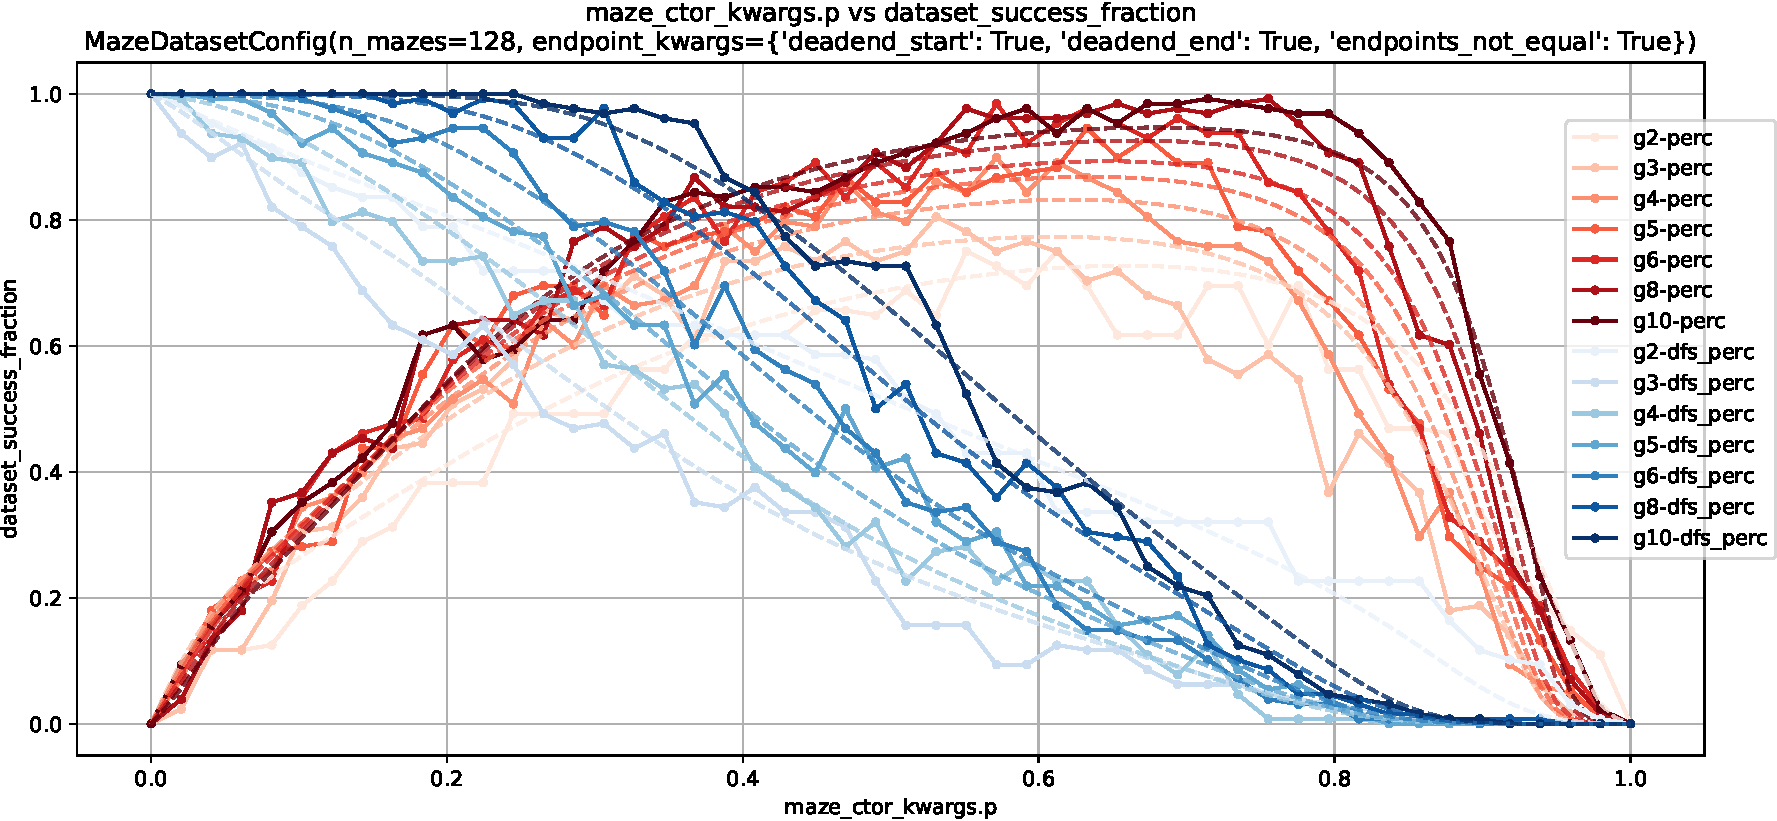
\includegraphics[width=1\textwidth,height=\textheight]{figures/ep/ep_deadends_unique-crop.pdf}
\caption{An example of both empirical and predicted success rates as a
function of the percolation probability \(p\) for various maze sizes,
percolation with and without depth first search, and
\texttt{endpoint\_kwargs} requiring that both the start and end be in
unique dead ends. Empirical measures derived from a sample of 128 mazes.
More information can be found on the
\href{https://understanding-search.github.io/maze-dataset/benchmarks/}{benchmarks
page}.}
\end{figure}

\hypertarget{sec:implementation}{%
\section{Implementation}\label{sec:implementation}}

We refer to our
\href{https://github.com/understanding-search/maze-dataset}{repository}
and
\href{https://understanding-search.github.io/maze-dataset/maze_dataset.html}{docs}
for documentation and up-to-date implementation details.

This package utilizes a simple, efficient representation of mazes as
subgraphs of a finite lattice, which we call a
\href{https://understanding-search.github.io/maze-dataset/maze_dataset.html\#LatticeMaze}{\texttt{LatticeMaze}}.
Using an adjacency matrix for storing mazes would be memory inefficient
by failing to exploit the highly sparse structure -- for example, for a
2-dimensional maze, only 4 of the diagonals would be filled in. On the
other hand, using an adjacency list could lead to a poor lookup time for
whether any given connection exists.

Instead, we describe mazes with the following representation: for a
\(2\)-dimensional lattice with \(r\) rows and \(c\) columns, we
initialize a boolean array \[
  A = \{0, 1\}^{2 \times r \times c}
\] which we refer to in the code as a
\href{https://understanding-search.github.io/maze-dataset/maze_dataset.html\#LatticeMaze.connection_list}{\texttt{connection\_list}}.
The value at \(A[0,i,j]\) determines whether a \emph{downward}
connection exists from node \([i,j]\) to \([i+1, j]\). Likewise, the
value at \(A[1,i,j]\) determines whether a \emph{rightward} connection
to \([i, j+1]\) exists. Thus, we avoid duplication of data about the
existence of connections and facillitate fast lookup time, at the cost
of requiring additional care with indexing. Note that this setup allows
for a periodic lattice. Generation of mazes is detailed in
\href{https://understanding-search.github.io/maze-dataset/maze_dataset.html\#LatticeMazeGenerators}{\texttt{LatticeMazeGenerators}}.

To produce solutions to mazes, two points are selected uniformly at
random without replacement from the connected component of the maze, and
the \(A^*\) algorithm (\protect\hyperlink{ref-A_star}{Hart et al.,
1968}) is applied to find the shortest path between them. The endpoint
selection can be controlled via
\href{https://understanding-search.github.io/maze-dataset/maze_dataset/dataset/maze_dataset_config.html\#MazeDatasetConfig.endpoint_kwargs}{\texttt{MazeDatasetConfig.endpoint\_kwargs:}}
\href{https://understanding-search.github.io/maze-dataset/maze_dataset/dataset/maze_dataset_config.html\#EndpointKwargsType}{\texttt{EndpointKwargsType}},
and complications caused by this are detailed in
\hyperref[sec:success-rate-estimation]{section: \textit{\nameref{sec:success-rate-estimation}}}.
A maze with a solution is denoted a
\href{https://understanding-search.github.io/maze-dataset/maze_dataset.html\#SolvedMaze}{\texttt{SolvedMaze}},
which inherits from
\href{https://understanding-search.github.io/maze-dataset/maze_dataset.html\#LatticeMaze}{\texttt{LatticeMaze}}.

Parallelization is implemented via the \texttt{multiprocessing} module
in the Python standard library, and parallel generation can be
controlled via keyword arguments to
\href{https://understanding-search.github.io/maze-dataset/maze_dataset.html\#MazeDataset.from_config}{\texttt{MazeDataset.from\_config()}}.

\newpage

\hypertarget{usage-in-research}{%
\section{Usage in Research}\label{usage-in-research}}

This package was originally built for the needs of the
(\protect\hyperlink{ref-maze-transformer-github}{Michael I. Ivanitskiy
et al., 2023b}) project, which aims to investigate spatial planning and
world models in autoregressive transformer models trained on mazes
(\protect\hyperlink{ref-ivanitskiy2023structuredworldreps}{Michael
Igorevich Ivanitskiy, Spies, et al., 2023};
\protect\hyperlink{ref-maze-dataset-arxiv-2023}{Michael Igorevich
Ivanitskiy, Shah, et al., 2023};
\protect\hyperlink{ref-spies2024causalworldmodels}{Spies et al., 2024}).
It was extended for work on understanding the mechanisms by which
recurrent convolutional and implicit networks
(\protect\hyperlink{ref-fung2022jfb}{Fung et al., 2022}) solve mazes
given a rasterized view
(\protect\hyperlink{ref-knutson2024logicalextrapolation}{Knutson et al.,
2024}), which required matching the pixel-padded and endpoint
constrained output format of
(\protect\hyperlink{ref-easy_to_hard}{Schwarzschild, Borgnia, Gupta,
Bansal, et al., 2021}). Ongoing work using \texttt{maze-dataset} aims to
investigate the effects of varying the tokenization format on the
performance of pretrained LLMs on spatial reasoning.

This package has also been utilized in work by other groups:

\begin{itemize}
\item
  By (\protect\hyperlink{ref-nolte2024multistep}{Nolte et al., 2024}) to
  compare the effectiveness of transformers trained with the
  MLM-\(\mathcal{U}\)
  (\protect\hyperlink{ref-MLMU-kitouni2024factorization}{Kitouni et al.,
  2024}) multistep prediction objective against standard autoregressive
  training for multi-step planning on our maze task.
\item
  By (\protect\hyperlink{ref-wang2024imperative}{Wang et al., 2024}) and
  (\protect\hyperlink{ref-chen2024iaimperative}{Chen et al., 2024}) to
  study the effectiveness of imperative learning.
\item
  By (\protect\hyperlink{ref-zhang2025tscend}{Zhang et al., 2025}) to
  introduce a novel framework for reasoning diffusion models.
\item
  By (\protect\hyperlink{ref-dao2025alphamaze}{Dao \& Vu, 2025}) to
  improve spatial reasoning in LLMs with GRPO.
\end{itemize}

\hypertarget{acknowledgements}{%
\section{Acknowledgements}\label{acknowledgements}}

This work was partially funded by National Science Foundation awards
DMS-2110745 and DMS-2309810. We are also grateful to LTFF and FAR Labs
for hosting authors MII, AFS, and TR for a residency visit, and to
various members of FAR's technical staff for their advice.

This work was partially supported by AI Safety Camp and AI Safety
Support, which also brought many of the authors together. We would like
to thank our former collaborators at AI Safety Camp and other users and
contributors to the \texttt{maze-dataset} package: Benji Berczi,
Guillaume Corlouer, William Edwards, Leon Eshuijs, Chris Mathwin, Lucia
Quirke, Can Rager, Adrians Skapars, Rusheb Shah, Johannes Treutlein, and
Dan Valentine.

We thank the Mines Optimization and Deep Learning group (MODL) for
fruitful discussions. We also thank Michael Rosenberg for recommending
the usage of Finite State Transducers for storing tokenizer validation
information.

\newpage

\hypertarget{references}{%
\section*{References}\label{references}}
\addcontentsline{toc}{section}{References}

\hypertarget{refs}{}
\begin{CSLReferences}{1}{0.5}
\leavevmode\vadjust pre{\hypertarget{ref-mazegenerator-net}{}}%
Alance AB. (2019). \emph{Maze generator}.
\url{http://www.mazegenerator.net}.

\leavevmode\vadjust pre{\hypertarget{ref-ayaz2008maze}{}}%
Ayaz, H., Allen, S. L., Platek, S. M., \& Onaral, B. (2008). Maze suite
1.0: A complete set of tools to prepare, present, and analyze
navigational and spatial cognitive neuroscience experiments.
\emph{Behavior Research Methods}, \emph{40}, 353--359.

\leavevmode\vadjust pre{\hypertarget{ref-chen2024iaimperative}{}}%
Chen, X., Yang, F., \& Wang, C. (2024). {iA*}: Imperative learning-based
{A*} search for pathfinding. \emph{arXiv Preprint arXiv:2403.15870}.

\leavevmode\vadjust pre{\hypertarget{ref-cobbe2019procgen}{}}%
Cobbe, K., Hesse, C., Hilton, J., \& Schulman, J. (2019). Leveraging
procedural generation to benchmark reinforcement learning. \emph{arXiv
Preprint arXiv:1912.01588}.

\leavevmode\vadjust pre{\hypertarget{ref-pysr}{}}%
Cranmer, M. (2023). Interpretable machine learning for science with PySR
and SymbolicRegression. jl. \emph{arXiv Preprint arXiv:2305.01582}.

\leavevmode\vadjust pre{\hypertarget{ref-dao2025alphamaze}{}}%
Dao, A., \& Vu, D. B. (2025). AlphaMaze: Enhancing large language
models' spatial intelligence via GRPO. \emph{arXiv Preprint
arXiv:2502.14669}.

\leavevmode\vadjust pre{\hypertarget{ref-percolation}{}}%
Duminil-Copin, H. (2017). \emph{Sixty years of percolation} (No.
arXiv:1712.04651). {arXiv}. \url{http://arxiv.org/abs/1712.04651}

\leavevmode\vadjust pre{\hypertarget{ref-gh_Ehsan_2022}{}}%
Ehsan, E. (2022). \emph{Maze}. \url{https://github.com/emadehsan/maze}

\leavevmode\vadjust pre{\hypertarget{ref-percolation-clustersize}{}}%
Fisher, M. E., \& Essam, J. W. (2004). Some {Cluster Size} and
{Percolation Problems}. \emph{Journal of Mathematical Physics},
\emph{2}(4), 609--619. \url{https://doi.org/10.1063/1.1703745}

\leavevmode\vadjust pre{\hypertarget{ref-fung2022jfb}{}}%
Fung, S. W., Heaton, H., Li, Q., McKenzie, D., Osher, S., \& Yin, W.
(2022). Jfb: Jacobian-free backpropagation for implicit networks.
\emph{Proceedings of the AAAI Conference on Artificial Intelligence},
\emph{36}, 6648--6656.

\leavevmode\vadjust pre{\hypertarget{ref-mathematica-maze}{}}%
Guo, C., Barthelet, L., \& Morris, R. (2011). \emph{Maze generator and
solver}. Wolfram Demonstrations Project,
\url{https://demonstrations.wolfram.com/MazeGeneratorAndSolver/}.

\leavevmode\vadjust pre{\hypertarget{ref-harriesMazeExplorerCustomisable3D2019}{}}%
Harries, L., Lee, S., Rzepecki, J., Hofmann, K., \& Devlin, S. (n.d.).
{MazeExplorer}: {A Customisable 3D Benchmark} for {Assessing
Generalisation} in {Reinforcement Learning}. \emph{2019 {IEEE Conf}.
{Games CoG}}, 1--4.

\leavevmode\vadjust pre{\hypertarget{ref-A_star}{}}%
Hart, P. E., Nilsson, N. J., \& Raphael, B. (1968). A {Formal Basis} for
the {Heuristic Determination} of {Minimum Cost Paths}. \emph{IEEE
Transactions on Systems Science and Cybernetics}, \emph{4}(2), 100--107.
\url{https://doi.org/10.1109/TSSC.1968.300136}

\leavevmode\vadjust pre{\hypertarget{ref-zanj}{}}%
Ivanitskiy, M. (n.d.). \emph{ZANJ}.
\url{https://github.com/mivanit/ZANJ}

\leavevmode\vadjust pre{\hypertarget{ref-maze-dataset-github}{}}%
Ivanitskiy, Michael I., Shah, R., Spies, A. F., Räuker, T., Valentine,
D., Rager, C., Quirke, L., Corlouer, G., \& Mathwin, C. (2023a).
\emph{Maze dataset}.
\url{https://github.com/understanding-search/maze-dataset}

\leavevmode\vadjust pre{\hypertarget{ref-maze-transformer-github}{}}%
Ivanitskiy, Michael I., Shah, R., Spies, A. F., Räuker, T., Valentine,
D., Rager, C., Quirke, L., Corlouer, G., \& Mathwin, C. (2023b).
\emph{Maze transformer interpretability}.
\url{https://github.com/understanding-search/maze-transformer}

\leavevmode\vadjust pre{\hypertarget{ref-maze-dataset-arxiv-2023}{}}%
Ivanitskiy, Michael Igorevich, Shah, R., Spies, A. F., Räuker, T.,
Valentine, D., Rager, C., Quirke, L., Mathwin, C., Corlouer, G., Behn,
C. D., \& others. (2023). A configurable library for generating and
manipulating maze datasets. \emph{arXiv Preprint arXiv:2309.10498}.

\leavevmode\vadjust pre{\hypertarget{ref-ivanitskiy2023structuredworldreps}{}}%
Ivanitskiy, Michael Igorevich, Spies, A. F., Räuker, T., Corlouer, G.,
Mathwin, C., Quirke, L., Rager, C., Shah, R., Valentine, D., Behn, C.
D., \& others. (2023). Structured world representations in maze-solving
transformers. \emph{arXiv Preprint arXiv:2312.02566}.

\leavevmode\vadjust pre{\hypertarget{ref-MLMU-kitouni2024factorization}{}}%
Kitouni, O., Nolte, N. S., Williams, A., Rabbat, M., Bouchacourt, D., \&
Ibrahim, M. (2024). The factorization curse: Which tokens you predict
underlie the reversal curse and more. \emph{Advances in Neural
Information Processing Systems}, \emph{37}, 112329--112355.

\leavevmode\vadjust pre{\hypertarget{ref-knutson2024logicalextrapolation}{}}%
Knutson, B., Rabeendran, A. C., Ivanitskiy, M., Pettyjohn, J.,
Diniz-Behn, C., Fung, S. W., \& McKenzie, D. (2024). On logical
extrapolation for mazes with recurrent and implicit networks.
\emph{arXiv Preprint arXiv:2410.03020}.

\leavevmode\vadjust pre{\hypertarget{ref-kruskal1956shortest}{}}%
Kruskal, J. B. (1956). On the shortest spanning subtree of a graph and
the traveling salesman problem. \emph{Proceedings of the American
Mathematical Society}, \emph{7}(1), 48--50.

\leavevmode\vadjust pre{\hypertarget{ref-eval-LLM-graphs}{}}%
Liu, C., \& Wu, B. (2023). Evaluating large language models on graphs:
Performance insights and comparative analysis. \emph{arXiv Preprint
arXiv:2308.11224}.

\leavevmode\vadjust pre{\hypertarget{ref-mdl-suite}{}}%
Nag, A. (2020). MDL suite: A language, generator and compiler for
describing mazes. \emph{Journal of Open Source Software}, \emph{5}(46),
1815.

\leavevmode\vadjust pre{\hypertarget{ref-gh_Nemeth_2019}{}}%
Németh, F. (2019). \emph{Maze-generation-algorithms}.
\url{https://github.com/ferenc-nemeth/maze-generation-algorithms}

\leavevmode\vadjust pre{\hypertarget{ref-nolte2024multistep}{}}%
Nolte, N., Kitouni, O., Williams, A., Rabbat, M., \& Ibrahim, M. (2024).
Transformers can navigate mazes with multi-step prediction. \emph{arXiv
Preprint arXiv:2412.05117}.

\leavevmode\vadjust pre{\hypertarget{ref-gh-oppenheimj2018maze}{}}%
Oppenheim, J. (2018). \emph{Maze-generator: Generate a random maze
represented as a 2D array using depth-first search}.
\url{https://github.com/oppenheimj/maze-generator/}; GitHub.

\leavevmode\vadjust pre{\hypertarget{ref-pytorch}{}}%
Paszke, A., Gross, S., Massa, F., Lerer, A., Bradbury, J., Chanan, G.,
Killeen, T., Lin, Z., Gimelshein, N., Antiga, L., Desmaison, A., Kopf,
A., Yang, E., DeVito, Z., Raison, M., Tejani, A., Chilamkurthy, S.,
Steiner, B., Fang, L., \ldots{} Chintala, S. (2019). {PyTorch: An
Imperative Style, High-Performance Deep Learning Library}. In H.
Wallach, H. Larochelle, A. Beygelzimer, F. d'Alché-Buc, E. Fox, \& R.
Garnett (Eds.), \emph{Advances in neural information processing systems
32} (pp. 8024--8035). Curran Associates, Inc.
\url{http://papers.neurips.cc/paper/9015-pytorch-an-imperative-style-high-performance-deep-learning-library.pdf}

\leavevmode\vadjust pre{\hypertarget{ref-pfau2024dotbydot}{}}%
Pfau, J., Merrill, W., \& Bowman, S. R. (2024). Let's think dot by dot:
Hidden computation in transformer language models. \emph{arXiv Preprint
arXiv:2404.15758}.

\leavevmode\vadjust pre{\hypertarget{ref-interpretability-survery}{}}%
Räuker, T., Ho, A., Casper, S., \& Hadfield-Menell, D. (2023). Toward
transparent ai: A survey on interpreting the inner structures of deep
neural networks. \emph{2023 IEEE Conference on Secure and Trustworthy
Machine Learning (SaTML)}, 464--483.

\leavevmode\vadjust pre{\hypertarget{ref-easy_to_hard}{}}%
Schwarzschild, A., Borgnia, E., Gupta, A., Bansal, A., Emam, Z., Huang,
F., Goldblum, M., \& Goldstein, T. (2021). \emph{Datasets for {Studying
Generalization} from {Easy} to {Hard Examples}} (No. arXiv:2108.06011).
{arXiv}. \url{https://doi.org/10.48550/arXiv.2108.06011}

\leavevmode\vadjust pre{\hypertarget{ref-deepthinking}{}}%
Schwarzschild, A., Borgnia, E., Gupta, A., Huang, F., Vishkin, U.,
Goldblum, M., \& Goldstein, T. (2021). Can you learn an algorithm?
Generalizing from easy to hard problems with recurrent networks.
\emph{Advances in Neural Information Processing Systems}, \emph{34},
6695--6706.

\leavevmode\vadjust pre{\hypertarget{ref-eval-gpt-visual}{}}%
Singla, A. (2023). Evaluating ChatGPT and GPT-4 for visual programming.
\emph{arXiv Preprint arXiv:2308.02522}.

\leavevmode\vadjust pre{\hypertarget{ref-spies2024causalworldmodels}{}}%
Spies, A. F., Edwards, W., Ivanitskiy, M. I., Skapars, A., Räuker, T.,
Inoue, K., Russo, A., \& Shanahan, M. (2024). Transformers use causal
world models in maze-solving tasks. \emph{arXiv Preprint
arXiv:2412.11867}.

\leavevmode\vadjust pre{\hypertarget{ref-wang2024imperative}{}}%
Wang, C., Ji, K., Geng, J., Ren, Z., Fu, T., Yang, F., Guo, Y., He, H.,
Chen, X., Zhan, Z., \& others. (2024). Imperative learning: A
self-supervised neural-symbolic learning framework for robot autonomy.
\emph{arXiv Preprint arXiv:2406.16087}.

\leavevmode\vadjust pre{\hypertarget{ref-wilson}{}}%
Wilson, D. B. (1996). Generating random spanning trees more quickly than
the cover time. \emph{Proceedings of the Twenty-Eighth Annual {ACM}
Symposium on {Theory} of Computing - {STOC} '96}, 296--303.
\url{https://doi.org/10.1145/237814.237880}

\leavevmode\vadjust pre{\hypertarget{ref-zhang2025tscend}{}}%
Zhang, T., Pan, J.-S., Feng, R., \& Wu, T. (2025). T-SCEND: Test-time
scalable MCTS-enhanced diffusion model. \emph{arXiv Preprint
arXiv:2502.01989}.

\end{CSLReferences}

\end{document}
